% Load the preamble which handles package loading and configuration
% Document Class Configuration
\documentclass[12pt, a4paper]{report} % Removed 'most' option (belongs to tcolorbox)
\title{Modélisation du Trafic Routier au Bénin}
\author{AHOUANYE Elonm}
\date{\today}

% Preamble for memoire.tex - Centralized package management
% Organized by category for clarity




% --- Input Encoding & Language ---
\usepackage[utf8]{inputenc}   % Required for special characters (only if using pdfLaTeX)
% \usepackage[T1]{fontenc}    % Removed - not needed with XeLaTeX/LuaLaTeX
% Choose only one language system:
% \usepackage[french]{babel}  % Commented out to avoid conflict
\usepackage{polyglossia}      % Advanced multilingual support
\setmainlanguage{french}      % Set default language

% --- Mathematics Packages ---
\usepackage{bm} % Bold Math
\usepackage{algorithm}
\usepackage{algpseudocode}
\usepackage{amsmath, amssymb, amsfonts} % AMS math packages
\usepackage{amsthm}          % Required for thmtools
\usepackage{mathtools}        % Extends amsmath
\usepackage{thmtools}         % For theorem environments
\usepackage{empheq}           % For boxed equations
\usepackage{unicode-math}     % Unicode math support
\setmathfont{TeX Gyre Pagella Math}

% --- Layout & Formatting ---
\usepackage{geometry}         % Page layout control
\geometry{
  top=2.5cm,
  bottom=2.5cm,
  left=2.5cm,
  right=2.5cm,
  marginparwidth=1.8cm,
  marginparsep=0.3cm,
  headsep=0.7cm,
  footskip=1.2cm,
  headheight=30pt  % Increased to fix warnings
}
\usepackage{setspace}         % Line spacing
\usepackage{fancyhdr}         % Custom headers/footers
\usepackage{titlesec}         % Section title formatting

% --- Graphics & Figures ---
\usepackage{graphicx}         % Include graphics
\usepackage{subcaption}       % Sub-figures
\usepackage{float}            % Improved figure positioning
\graphicspath{{images/}{simulations/}} % Graphics path

% --- Tables & Lists ---
\usepackage{booktabs}         % Professional tables
\usepackage{longtable}        % Multi-page tables
\usepackage{colortbl}         % Colored table cells/rows
\usepackage{multirow}        % Multi-row cells in tables
\usepackage{array}            % Extended table functionality
\usepackage{enumitem}         % Customizable lists

% --- Code & Listings ---
\usepackage{listings}         % Code listings (if needed)
\usepackage{xcolor}           % Color support (used by listings, tcolorbox, etc.)
\usepackage[most]{tcolorbox}  % Moved 'most' option here where it belongs
% \tcbuselibrary{most}        % Removed as redundant with the option above

% --- References & Citations ---
\usepackage{hyperref}         % Hyperlinks in PDF
\hypersetup{
    colorlinks=true,
    linkcolor=blue, % Changed to blue for consistency
    filecolor=blue,      
    urlcolor=blue,
    citecolor=blue,
    pdftitle={Modélisation du Trafic Routier au Bénin},
    pdfauthor={Votre Nom},
    pdfkeywords={trafic routier, Bénin, modèle LWR, motos, multiclasses},
}
\usepackage{cleveref}         % Intelligent cross-referencing
\usepackage{nameref}          % Named references
\usepackage{zref-abspage}     % Absolute page numbers
\usepackage{rerunfilecheck}   % Check for outdated auxiliary files

% --- Other Packages ---
\usepackage{verbatim}         % Verbatim environment
\usepackage{environ}          % Environment manipulation
\usepackage{trimspaces}       % Trim spaces around tokens
\usepackage{etoolbox}         % e-TeX tools
\usepackage{mdframed}         % Framed environments
\usepackage{kvoptions}        % Key-value options
\usepackage{ltxcmds}          % LaTeX kernel commands
\usepackage{kvsetkeys}        % Key-value parser
\usepackage{infwarerr}        % Info/warning/error messages
\usepackage{kvdefinekeys}     % Define keys
\usepackage{pdftexcmds}       % Utility functions of pdfTeX
\usepackage{etexcmds}         % Avoid name clashes with e-TeX commands
\usepackage{auxhook}          % Hooks for auxiliary files
\usepackage{needspace}        % Reserve vertical space
\usepackage{pgfplots}         % Create plots
\pgfplotsset{compat=1.18}     % Set PGFPlots compatibility level
\usepackage{pgfplotstable}    % Table support for PGFPlots
\usepackage{xkeyval}          % Key-value package
\usepackage{adjustbox}        % Adjusting TeX boxes
\usepackage{ifoddpage}        % Check for odd/even page
\usepackage{varwidth}         % Variable-width minipages
% \usepackage{sidenotes}        % Temporarily disabled for debugging
\usepackage{marginnote}       % Non-floating margin notes
\usepackage{changepage}       % Change page layout
% \usepackage{csvsimple}        % Temporarily disabled for debugging

% --- Simplified glossaries setup ---
\PassOptionsToPackage{math=fp}{datatool} % Use fp math engine for datatool compatibility
\usepackage[acronym]{glossaries} % Temporarily disabled for debugging
% Option nohypertypes avoids issues with datatool

% Note: \PassOptionsToPackage for datatool moved above \usepackage{glossaries}
%\PassOptionsToPackage{math=l3fp}{datatool} % l3fp can sometimes cause issues



\usepackage{mfirstuc}         % Temporarily disabled for debugging
\usepackage{xfor}             % Temporarily disabled for debugging
\usepackage{tracklang}        % Temporarily disabled for debugging
\usepackage{imakeidx}         % Moved below bookmark
\usepackage{multicol}         % Temporarily disabled for debugging
\usepackage{bookmark}         % Moved below
\usepackage{imakeidx}         % Temporarily disabled for debugging
% --- Font Configuration ---
\setmainfont{TeX Gyre Pagella}[
  Numbers=OldStyle,
  Ligatures=TeX
]
\setsansfont{TeX Gyre Heros}[Scale=0.9]
\setmonofont{Fira Mono}[Scale=0.85] % Changed from Fira Mono for debugging

% --- Fix for fix-cm ---
\usepackage{fix-cm}  % Not needed with XeLaTeX/LuaLaTeX

% --- Load custom commands and styles ---
% Check if this file exists before uncommenting:
\usepackage{styles/benintraffic}

\usepackage{bookmark}         % Temporarily disabled for debugging
% --- Glossary ---
\makeglossaries

% Comment this line if this is being included in another document:

% Load book class commands for front/main/backmatter
\makeatletter
\@ifundefined{@mainmatter}{%
  \newif\if@mainmatter \@mainmattertrue
}{}
\@ifundefined{frontmatter}{%
  \newcommand\frontmatter{%
    \cleardoublepage
    \@mainmatterfalse
    \pagenumbering{roman}}%
}{}
\@ifundefined{mainmatter}{%
  \newcommand\mainmatter{%
    \cleardoublepage
    \@mainmattertrue
    \pagenumbering{arabic}}%
}{}
\@ifundefined{backmatter}{%
  \newcommand\backmatter{%
    \if@openright\cleardoublepage\else\clearpage\fi
    \@mainmatterfalse}%
}{}
\makeatother

% Graphics path
\graphicspath{{images/}{simulations/}}

% Custom styles
\usepackage{styles/benintraffic}
\usepackage{imakeidx} % Already loaded in preamble.tex
% \makeindex % imakeidx should handle this automatically

\begin{document}

\maketitle

% Front matter
\frontmatter
\begin{titlepage}
\thispagestyle{empty}
\pagecolor{white} % Ensure white background for cover

\begin{center}

% University logo or emblem
\vspace*{-1cm}

\includegraphics[width=3.5cm]{images/logo-university.jpg}\\[0.5cm]

\textsc{\Large Université Nationale Supérieure de Technologie, Ingénierie et Mathématiques}\\[0.3cm]
\textsc{\large École Nationale Supérieure de Génie Mathématique et Modélisation}\\[0.2cm]
\textsc{\large ENSGMM}\\[1.5cm]

% Thesis type and program
\textsc{\large Mémoire de Master}\\
\textsc{\normalsize Spécialité: Mathématiques Appliquées}\\[2cm]

% Title with decorative rules
{\color{darkblue}\rule{\textwidth}{1.5pt}}\\[0.45cm]
{\LARGE\bfseries\color{darkblue}Modélisation du Trafic Routier au Bénin:\\[0.2cm]
\large Approche Macroscopique et Extension du Modèle LWR}\\[0.45cm]
{\color{darkblue}\rule{\textwidth}{1.5pt}}\\[1.5cm]

% Optional: Traffic-related decorative graphic
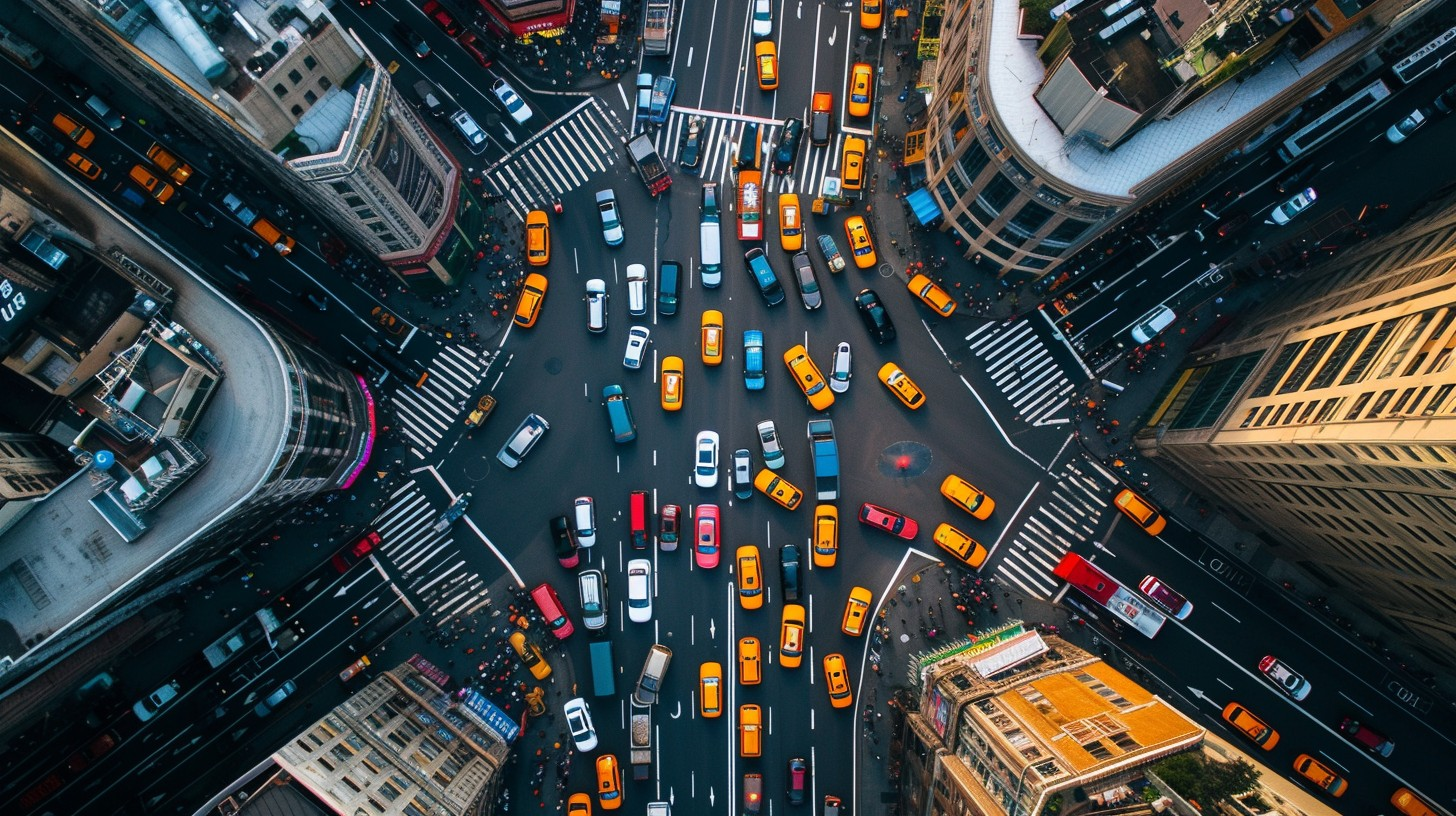
\includegraphics[width=8cm]{images/traffic-graphic.jpg}\\[1.2cm]

% Author information
\begin{flushright}
\large
\emph{Présenté par:}\\
\textbf{Votre Nom}\\[1cm]
\emph{Sous la direction de:}\\
\textbf{Pr. Directeur de Thèse}\\
\end{flushright}

\vfill

% Bottom date and place
{\large\bfseries Cotonou, \today}

\end{center}
\end{titlepage}
\pagecolor{pagebackground} % Reset to document background color

\chapter*{Dédicace}
\thispagestyle{empty}

\vspace*{2cm}

\begin{flushright}
\emph{Je dédie ce travail à...}

\vspace{1cm}

Ma famille, pour leur soutien indéfectible...

\vspace{1cm}

Les usagers des routes béninoises, dont les comportements 
et adaptations m'ont inspiré cette recherche...

\vspace{1cm}

Et à tous ceux qui œuvrent pour améliorer 
la mobilité urbaine en Afrique de l'Ouest.
\end{flushright}

\vspace*{\fill}

\chapter*{Remerciements}
\thispagestyle{empty}

Je tiens à exprimer ma profonde gratitude à toutes les personnes qui ont contribué, directement ou indirectement, à la réalisation de ce travail de recherche.

\vspace{0.5cm}

Mes remerciements vont tout d'abord à mon directeur de mémoire, \textbf{Pr. [Nom du Directeur]}, pour sa disponibilité, ses conseils avisés et son encadrement rigoureux tout au long de cette étude.

\vspace{0.5cm}

Je souhaite également remercier \textbf{[Nom]}, \textbf{[Nom]} et \textbf{[Nom]} pour leur contribution à la collecte des données de terrain et pour le partage de leurs connaissances approfondies du réseau routier béninois.

\vspace{0.5cm}

Ma reconnaissance s'adresse aussi au personnel de \textbf{l'Institut de Mathématiques et de Sciences Physiques (IMSP)} pour le cadre propice à la recherche qu'ils offrent aux étudiants.

\vspace{0.5cm}

Je suis particulièrement reconnaissant envers les conducteurs de zémidjans et les chauffeurs professionnels qui ont accepté de participer aux entretiens et enquêtes, fournissant ainsi des informations précieuses sur les comportements de conduite spécifiques au Bénin.

\vspace{0.5cm}

Enfin, mes remerciements vont à ma famille et à mes amis pour leur patience et leur soutien moral durant cette période d'intense travail.

\chapter*{Résumé}
\thispagestyle{empty}

Ce mémoire propose une extension du modèle macroscopique de trafic LWR (Lighthill-Whitham-Richards) adaptée aux spécificités du réseau routier béninois. Le système de transport au Bénin présente des caractéristiques uniques : prédominance des motos (Zémidjans), hétérogénéité des infrastructures routières, et comportements de conduite particuliers qui ne sont pas correctement représentés par les modèles traditionnels.

Notre approche introduit un modèle multiclasses intégrant explicitement le comportement des motos et leur interaction avec les autres véhicules. Nous définissons des fonctions de modulation spécifiques $f_{M,i}(\rho_M)$ qui quantifient l'impact des motos sur l'écoulement du trafic, notamment les phénomènes de gap-filling et d'interweaving. De plus, nous intégrons l'influence variable du revêtement routier sur la vitesse des différentes classes de véhicules à travers un coefficient de ralentissement $\lambda_{\text{mat},i}$.

Le modèle est calibré et validé sur des données réelles collectées sur le réseau routier béninois. Les résultats démontrent sa capacité à représenter fidèlement les dynamiques locales, notamment aux intersections et dans les zones de congestion. Une analyse de sensibilité identifie les paramètres les plus influents et quantifie l'incertitude associée.

Cette extension du modèle LWR constitue un outil précieux pour la planification du trafic et l'évaluation des politiques de transport au Bénin, prenant en compte la réalité complexe de la circulation locale dominée par les deux-roues motorisés.

\vspace{1cm}

\noindent \textbf{Mots-clés :} modélisation du trafic, approche macroscopique, modèle LWR, trafic multiclasses, motos, Bénin, gap-filling, interweaving, coefficient de ralentissement, calibration, validation.

\chapter*{Abstract}
\thispagestyle{empty}

This thesis presents an extension of the LWR (Lighthill-Whitham-Richards) macroscopic traffic model adapted to the specific characteristics of Benin's road network. The transportation system in Benin exhibits unique features: predominance of motorcycles (Zemidjans), heterogeneity of road infrastructure, and particular driving behaviors that are not properly represented by traditional models.

Our approach introduces a multi-class model explicitly integrating motorcycle behavior and their interaction with other vehicles. We define specific modulation functions $f_{M,i}(\rho_M)$ that quantify the impact of motorcycles on traffic flow, including gap-filling and interweaving phenomena. Additionally, we incorporate the variable influence of road surface quality on the speed of different vehicle classes through a slowing coefficient $\lambda_{\text{mat},i}$.

The model is calibrated and validated using real data collected from Benin's road network. Results demonstrate its ability to faithfully represent local dynamics, particularly at intersections and in congested areas. A sensitivity analysis identifies the most influential parameters and quantifies the associated uncertainty.

This extension of the LWR model provides a valuable tool for traffic planning and transportation policy evaluation in Benin, accounting for the complex reality of local traffic dominated by two-wheeled motorized vehicles.

\vspace{1cm}

\noindent \textbf{Keywords:} traffic modeling, macroscopic approach, LWR model, multi-class traffic, motorcycles, Benin, gap-filling, interweaving, slowing coefficient, calibration, validation.


\tableofcontents
\listoffigures
\listoftables

% Print glossary if needed
\printglossary[title=Glossaire des Termes]
\chapter*{Liste des Abréviations}
\addcontentsline{toc}{chapter}{Liste des Abréviations}
\thispagestyle{fancy}

\begin{tabular}{ll}
\toprule
\textbf{Abréviation} & \textbf{Signification} \\
\midrule
EDP & Équation aux Dérivées Partielles \\
GEH & Geoffrey E. Havers (statistique de validation du trafic) \\
IMSP & Institut de Mathématiques et de Sciences Physiques \\
LWR & Lighthill-Whitham-Richards (modèle macroscopique de trafic) \\
MAE & Mean Absolute Error (Erreur Absolue Moyenne) \\
MC & Monte Carlo (méthode de simulation) \\
RMSE & Root Mean Square Error (Erreur Quadratique Moyenne) \\
SIG & Système d'Information Géographique \\
UAC & Université d'Abomey-Calavi \\
véh/km & Véhicules par kilomètre (unité de densité de trafic) \\
véh/h & Véhicules par heure (unité de flux de trafic) \\
CFL & Courant-Friedrichs-Lewy \\
CTM & Cell Transmission Model (Modèle de Transmission Cellulaire) \\
PDE & Partial Differential Equation \\
HOV & High Occupancy Vehicle (Véhicule à Occupation Élevée) \\
HLL & Harten-Lax-van Leer (solveur numérique) \\
WENO & Weighted Essentially Non-Oscillatory (schéma numérique) \\
TVD & Total Variation Diminishing (schéma à variation totale décroissante) \\
INSAE & Institut National de la Statistique et de l'Analyse Économique (Bénin) \\
AERC & African Economic Research Consortium \\
\bottomrule
\end{tabular}

\vspace{1cm}

\begin{tabular}{ll}
\toprule
\textbf{Symbole} & \textbf{Description} \\
\midrule
$\rho, \dens$ & Densité du trafic \\
$v, \vel$ & Vitesse du trafic \\
$q, \flow$ & Flux du trafic \\
$\rho_i, \densi{i}$ & Densité de la classe $i$ de véhicules \\
$\rho_M, \densM$ & Densité des motos \\
$\lambda_{\text{mat},i}$ & Coefficient de ralentissement lié au revêtement pour la classe $i$ \\
$f_{M,i}$ & Fonction de modulation de l'effet des motos sur la classe $i$ \\
$\eta_M$ & Coefficient de gap-filling pour les motos \\
$\mu_i$ & Coefficient d'interweaving pour la classe $i$ \\
$S_i(x,t)$ & Terme source/puits pour la classe $i$ à la position $x$ et au temps $t$ \\
$\Delta q$ & Variation du flux à une intersection \\
\bottomrule
\end{tabular}


% Main content
\mainmatter

\chapter{Introduction}
\label{chap:introduction}

\section{Contexte et Problématique}
\label{sec:contexte}

La modélisation du trafic routier est devenue un outil essentiel pour la planification et la gestion des infrastructures de transport dans le monde entier. Cependant, les modèles traditionnels, développés principalement dans le contexte des pays industrialisés, se heurtent à des limites importantes lorsqu'ils sont appliqués aux réalités des pays en développement, et particulièrement au Bénin.

\subsection{Importance de la Modélisation du Trafic}
\label{subsec:importance}

La modélisation du trafic routier offre plusieurs avantages fondamentaux pour le développement et la gestion des infrastructures :

\begin{itemize}
\item Elle permet d'\textbf{anticiper les congestions} et d'optimiser les flux de véhicules;
\item Elle constitue un \textbf{outil d'aide à la décision} pour les investissements routiers;
\item Elle facilite l'\textbf{évaluation des impacts} environnementaux et économiques des politiques de transport;
\item Elle contribue à l'\textbf{amélioration de la sécurité routière} par l'identification des points critiques du réseau.
\end{itemize}

Dans un contexte de croissance urbaine rapide comme celui du Bénin, ces outils deviennent particulièrement précieux pour accompagner un développement durable des infrastructures.

\subsection{Défis Spécifiques au Bénin}
\label{subsec:defis_benin}

Le réseau routier béninois présente des particularités qui rendent inadéquate l'application directe des modèles classiques de trafic :

\begin{itemize}
\item \textbf{Hétérogénéité marquée du trafic} : coexistence de véhicules aux caractéristiques très différentes (voitures, camions, bus, et surtout motos);
\item \textbf{Prédominance des motos} (localement appelées Zémidjans lorsqu'elles servent de taxi), représentant plus de 70\% du parc automobile, avec des comportements de conduite spécifiques;
\item \textbf{Diversité des infrastructures routières} : routes bitumées, en terre, pavées, pistes informelles, souvent en état de dégradation variable;
\item \textbf{Comportements de conduite adaptés aux contraintes locales}, notamment les pratiques de gap-filling et d'interweaving des motos;
\item \textbf{Réglementation routière appliquée de manière variable} et présence importante de négociations informelles aux intersections.
\end{itemize}

\begin{figure}[htbp]
\centering
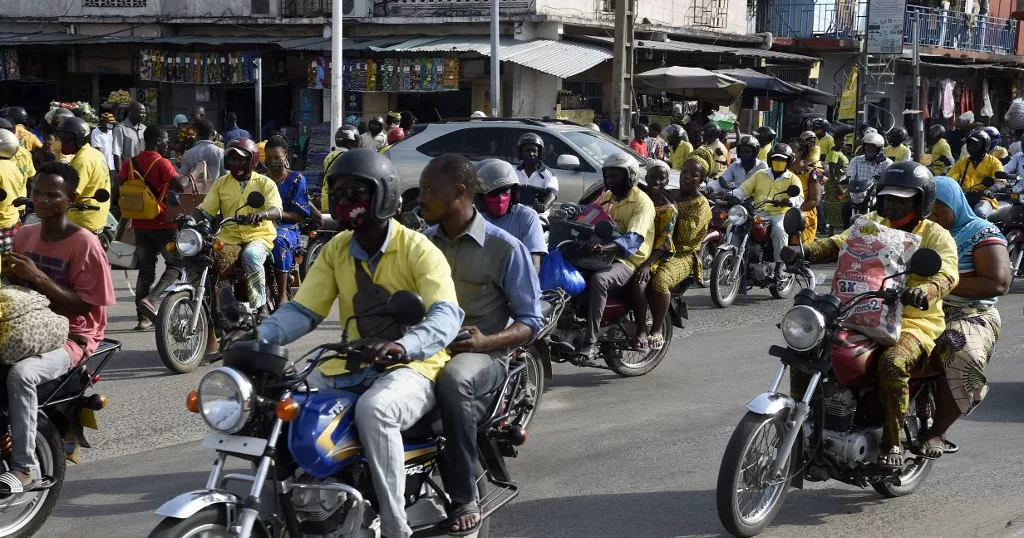
\includegraphics[width=0.8\textwidth]{images/introduction/trafic_cotonou}
\caption{Trafic typique à Cotonou montrant la prédominance des motos (Zémidjans) et leur comportement spécifique dans la circulation.}
\label{fig:trafic_cotonou}
\end{figure}

\subsection{Limites des Modèles Classiques}
\label{subsec:limites_modeles}

Le modèle LWR (Lighthill-Whitham-Richards), largement utilisé pour la modélisation macroscopique du trafic, repose sur plusieurs hypothèses qui s'avèrent inadaptées au contexte béninois :

\begin{itemize}
\item \textbf{Homogénéité des véhicules} : le modèle standard suppose une flotte uniforme, ce qui est très éloigné de la réalité béninoise;
\item \textbf{Relation vitesse-densité unique} : cette relation ne tient pas compte des différences de comportement entre classes de véhicules;
\item \textbf{Impact du revêtement routier négligé} : la qualité variable des routes influence pourtant significativement la dynamique du trafic;
\item \textbf{Absence de modélisation des comportements spécifiques} comme le gap-filling des motos;
\item \textbf{Traitement inadéquat des intersections} qui constituent des points névralgiques dans le réseau béninois.
\end{itemize}

Face à ces limites, il devient nécessaire de développer une extension du modèle LWR spécifiquement adaptée au contexte béninois.

\section{Objectifs de l'Étude}
\label{sec:objectifs}

Cette recherche vise à développer un modèle macroscopique de trafic routier adapté aux spécificités du Bénin, en poursuivant les objectifs suivants :

\begin{enumerate}
\item \textbf{Adapter le modèle LWR au contexte béninois} en préservant sa robustesse mathématique et sa simplicité relative;
\item \textbf{Intégrer la diversité des classes de véhicules}, avec une attention particulière aux motos et à leur comportement spécifique;
\item \textbf{Prendre en compte l'impact des infrastructures routières} sur la dynamique du trafic, notamment la qualité variable du revêtement;
\item \textbf{Modéliser efficacement les intersections} et autres singularités du réseau routier béninois;
\item \textbf{Développer un outil opérationnel} pour la planification et la gestion du trafic routier au Bénin;
\item \textbf{Valider le modèle avec des données locales} collectées sur le terrain.
\end{enumerate}

Ces objectifs s'inscrivent dans une démarche plus large visant à améliorer la compréhension et la gestion des systèmes de transport dans les pays en développement, en tenant compte de leurs spécificités.

\section{Contributions de l'Étude}
\label{sec:contributions}

Cette étude apporte plusieurs contributions significatives à la modélisation du trafic routier :

\subsection{Contributions Théoriques}
\label{subsec:contrib_theoriques}

\begin{itemize}
\item \textbf{Extension multiclasses du modèle LWR} intégrant des équations de conservation couplées pour chaque type de véhicule;
\item \textbf{Introduction d'un coefficient de ralentissement} $\lambda_{\text{mat},i}$ lié au revêtement routier pour chaque classe de véhicule;
\item \textbf{Développement de fonctions de modulation} $f_{M,i}(\rho_M)$ pour représenter l'influence des motos sur les autres classes de véhicules;
\item \textbf{Formalisation mathématique} des phénomènes de gap-filling et d'interweaving observés dans le trafic béninois.
\end{itemize}

\subsection{Contributions Méthodologiques et Pratiques}
\label{subsec:contrib_pratiques}

\begin{itemize}
\item \textbf{Méthodes de calibration spécifiques} pour les paramètres du modèle à partir de données réelles du Bénin;
\item \textbf{Techniques de validation adaptées} au contexte des pays en développement, où les données peuvent être parcellaires;
\item \textbf{Analyses de sensibilité quantitatives} permettant d'identifier les paramètres les plus influents du modèle;
\item \textbf{Cadre d'application opérationnel} pour l'utilisation du modèle dans la planification des infrastructures au Bénin.
\end{itemize}

Ces contributions visent à combler un vide important dans la littérature scientifique, où les modèles de trafic sont rarement adaptés aux spécificités des pays en développement, et particulièrement à la prévalence des deux-roues motorisés.

\section{Structure du Document}
\label{sec:structure}

Pour présenter notre travail de manière claire et structurée, ce document est organisé comme suit :

\begin{itemize}
\item Le \textbf{Chapitre \ref{chap:fondements_theoriques}} présente les fondements théoriques du modèle LWR standard, ses équations, ses propriétés mathématiques et ses limites.

\item Le \textbf{Chapitre \ref{chap:specificites_benin}} analyse en détail les spécificités du réseau routier béninois et le rôle particulier des motos dans la dynamique du trafic local.

\item Le \textbf{Chapitre \ref{chap:extension_modele}} développe notre extension du modèle LWR, avec l'approche multiclasses, les fonctions de modulation pour les motos, et le coefficient de ralentissement lié au revêtement.

\item Le \textbf{Chapitre \ref{chap:calibrage_validation}} présente les méthodes et résultats de calibration et de validation du modèle à partir de données collectées sur le terrain au Bénin.

\item Le \textbf{Chapitre \ref{chap:analyse_sensibilite}} propose une analyse de sensibilité des paramètres du modèle pour évaluer leur impact relatif sur les prédictions.

\item Le \textbf{Chapitre \ref{chap:intersections}} approfondit la modélisation des intersections et des changements de voie, points critiques du réseau béninois.

\item Le \textbf{Chapitre \ref{chap:aspects_stochastiques}} intègre des aspects stochastiques et comportementaux pour améliorer la précision du modèle.

\item Le \textbf{Chapitre \ref{chap:discussion}} discute les forces et limites du modèle proposé et envisage des perspectives d'amélioration.

\item Le \textbf{Chapitre \ref{chap:conclusion}} synthétise les principales contributions et conclut sur l'importance d'adapter les modèles de trafic aux contextes spécifiques des pays en développement.
\end{itemize}

Cette structure progressive permet d'aborder le problème depuis ses fondements théoriques jusqu'aux applications pratiques, en mettant en lumière la spécificité du contexte béninois et les innovations apportées par notre extension du modèle LWR.

% !TEX root = ../memoire.tex
\chapter{Fondements Théoriques : Le Modèle LWR de Base}
\label{chap:fondements_theoriques}

\section{Principes du Modèle LWR}
\label{sec:principes_lwr}

Le modèle macroscopique de trafic routier développé indépendamment par Lighthill et Whitham \cite{lighthill1955kinematic} et Richards \cite{richards1956shock}, communément appelé modèle LWR, constitue l'un des fondements de la théorie moderne de l'écoulement du trafic. Ce modèle s'appuie sur trois principes fondamentaux :

\begin{itemize}
    \item Le \textbf{principe de conservation de la masse}  : Ce principe stipule que le nombre de véhicules est conservé, c'est-à-dire qu'il n'y a ni création ni disparition de véhicules sur le tronçon de route considéré. Mathématiquement, cela se traduit par une équation de continuité reliant la densité du trafic et le flux de véhicules.
    \item L'\textbf{hypothèse d'une relation fonctionnelle entre le flux et la concentration}  : Le modèle LWR repose sur l'hypothèse fondamentale qu'il existe une relation unique et déterministe entre le flux de trafic (le nombre de véhicules passant un point donné par unité de temps) et la concentration (la densité de véhicules sur la route). Cette relation est généralement représentée par un diagramme fondamental, qui peut varier en fonction des conditions de la route.
    \item Le \textbf{principe de l'écoulement continu} : Ce principe considère le trafic comme un fluide continu, ce qui permet d'appliquer les équations de la dynamique des fluides pour décrire son comportement macroscopique. Cette approche est valide lorsque le nombre de véhicules est suffisamment élevé pour que les fluctuations individuelles soient négligeables.
\end{itemize}

\begin{definition}[Approche continue du trafic]
    L'approche macroscopique considère le trafic comme un flux continu caractérisé par des variables agrégées (densité, vitesse moyenne, flux) plutôt que par les trajectoires individuelles des véhicules.
    \end{definition}
    
    Le modèle LWR repose sur plusieurs hypothèses simplificatrices :
    
    \begin{itemize}
        \item \textbf{Le trafic est homogène} : Cette hypothèse suppose que les caractéristiques de la route (nombre de voies, largeur, etc.) et le comportement des conducteurs sont uniformes sur le tronçon considéré.
        \item \textbf{Il existe une relation unique entre la densité et le flux} : Le modèle LWR postule une relation déterministe et statique entre la densité du trafic et le flux, généralement représentée par le diagramme fondamental.
        \item \textbf{Les effets d'inertie et de relaxation sont négligeables} : Le modèle suppose que les conducteurs réagissent instantanément aux changements de densité, sans délai ni inertie.
        \item \textbf{Il n'y a ni entrées ni sorties intermédiaires} : Le modèle de base considère un tronçon de route sans jonctions, entrées ou sorties intermédiaires, où les véhicules entrent à une extrémité et sortent à l'autre.
        \item \textbf{La vitesse est une fonction de la seule densité} : le modèle suppose que la vitesse des véhicules ne dépend que de la densité locale et non d'autres facteurs tels que l'historique du trafic ou les conditions en aval.
    \end{itemize}

Ces hypothèses, bien que restrictives, permettent d'obtenir un modèle mathématiquement tractable qui capture les phénomènes essentiels du trafic, notamment la formation et la propagation des congestions.

\section{Variables et Équation de Conservation}
\label{sec:equation_conservation}

Le modèle LWR s'articule autour de trois variables macroscopiques fondamentales, définies comme des fonctions continues de la position $x$ et du temps $t$ :

\begin{definition}[Variables macroscopiques]
\begin{itemize}
\item La \textbf{densité} $\dens(x,t)$ : nombre de véhicules par unité de longueur (véh/km);
\item La \textbf{vitesse moyenne} $\vel(x,t)$ : vitesse moyenne des véhicules à la position $x$ au temps $t$ (km/h);
\item Le \textbf{flux} $\flow(x,t) = \dens(x,t) \cdot \vel(x,t)$ : nombre de véhicules traversant un point par unité de temps (véh/h).
\end{itemize}
\end{definition}

L'équation fondamentale du modèle LWR est l'équation de conservation, issue du principe de conservation des véhicules :

\begin{empheq}[box=\colorbox{lightblue!15}]{align}
\pd{\dens}{t} + \pd{(\dens \vel)}{x} &= 0 \notag \\
\text{ou} \quad \pd{\dens}{t} + \pd{\flow}{x} &= 0
\label{eq:conservation_lwr}
\end{empheq}

Cette équation stipule que la variation temporelle de la densité (terme $\pd{\dens}{t}$) additionnée à la variation spatiale du flux (terme $\pd{\flow}{x}$ ou $\pd{(\dens \vel)}{x}$) doit être nulle en l'absence de sources ou de puits. **Elle exprime la conservation du nombre de véhicules : tout changement de densité en un point est dû à une différence de flux entre ce qui entre et ce qui sort de ce point.**

\begin{remark}
L'équation de conservation est une équation aux dérivées partielles (EDP) du premier ordre, de type hyperbolique. Cette nature hyperbolique est responsable de la formation d'ondes de choc dans le trafic, correspondant aux fronts de congestion. **Ces ondes de choc se produisent lorsque le trafic de faible densité rattrape un trafic plus dense et plus lent en aval**.
\end{remark}

\section{Diagramme Fondamental et Relation Vitesse-Densité}
\label{sec:diagramme_fondamental}

Pour résoudre l'équation de conservation du modèle LWR, il est nécessaire de spécifier la relation entre le flux $\flow$ (ou la vitesse $\vel$) et la densité $\dens$, connue sous le nom de \textit{relation fondamentale du trafic} ou \textit{diagramme fondamental}.

Le diagramme fondamental établit la relation entre la densité et le flux (ou la vitesse) du trafic. Cette relation est essentielle pour fermer le système d'équations et rendre l'équation de conservation soluble. **Il représente une simplification de la réalité, car il suppose une relation statique et déterministe entre ces variables macroscopiques**.

\subsection{Le Modèle de Greenshields}
\label{subsec:greenshields}

La relation la plus simple et la plus utilisée est celle proposée par Greenshields \cite{greenshields1935study}, qui postule une relation linéaire entre la vitesse et la densité :

\begin{empheq}[box=\colorbox{lightblue!15}]{align}
\vel(\dens) = \maxvel \left(1 - \frac{\dens}{\maxdens}\right)
\label{eq:greenshields_vitesse}
\end{empheq}

où $\maxvel$ représente la vitesse maximale (ou vitesse en flux libre) et $\maxdens$ la densité maximale (ou densité de blocage).

En utilisant le modèle de Greenshields, la relation entre le flux et la densité se dérive de la combinaison de la relation linéaire vitesse-densité avec la définition du flux:
$$\flow(\dens) = \dens \cdot \vel(\dens)$$

En substituant l'équation de vitesse de Greenshields, on obtient :
\begin{align}
\flow(\dens) &= \dens \cdot \maxvel \left(1 - \frac{\dens}{\maxdens}\right) \\
&= \maxvel \dens - \frac{\maxvel}{\maxdens} \dens^2
\label{eq:greenshields_flux}
\end{align}

Cette équation révèle une relation parabolique entre le flux et la densité. Le flux est nul lorsque la densité est nulle (route vide) ou égale à la densité maximale $\maxdens$ (congestion maximale, embouteillage). Le flux maximal, correspondant à la capacité de la route, est atteint lorsque la densité est égale à la moitié de la densité maximale.

\begin{figure}[htbp]
\centering
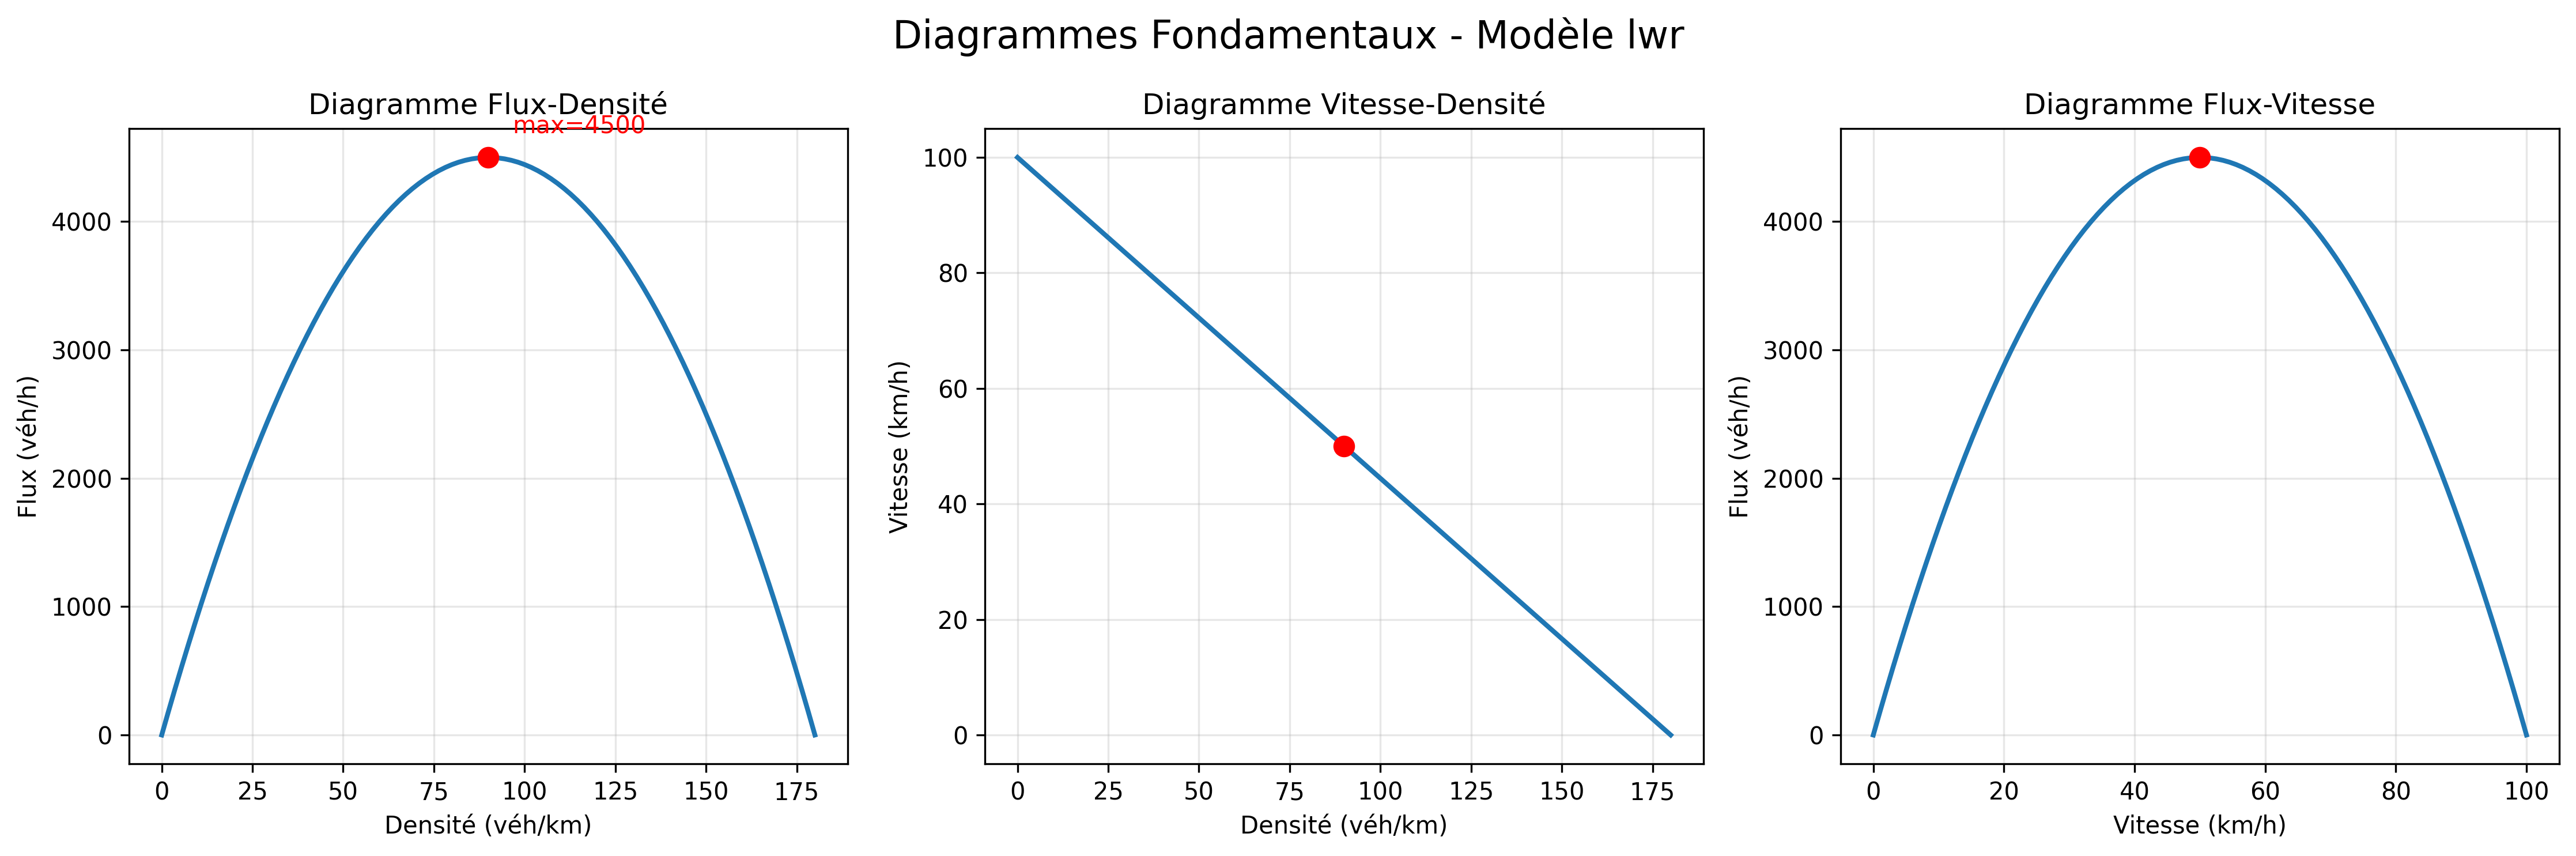
\includegraphics[width=1.0\textwidth]{simulations/LWR/diagrams/lwr_fundamental_diagrams}
\caption{Diagrammes fondamentaux du modèle LWR selon Greenshields : (a) relation vitesse-densité montrant la décroissance linéaire de la vitesse avec la densité, (b) relation flux-densité montrant la forme parabolique caractéristique avec le point critique à $\rho_c = \rho_{\text{max}}/2$, et (c) relation flux-vitesse.}
\label{fig:diagramme_fondamental}
\end{figure}

\subsection{Régimes de Circulation}
\label{subsec:regimes}

Le diagramme fondamental permet d'identifier trois régimes de circulation principaux :

\begin{enumerate}
    \item \textbf{Régime fluide (ou non congestionné)} : caractérisé par une faible densité, une vitesse élevée, et une augmentation du flux avec la densité. Dans ce régime, les véhicules peuvent circuler librement, et l'augmentation du nombre de véhicules sur la route entraîne une augmentation du flux total.
    \item \textbf{Régime critique} : correspond à une densité intermédiaire, où le flux atteint son maximum (capacité de la route). Ce point représente l'utilisation optimale de la route, où le nombre de véhicules est maximisé sans pour autant entraîner de congestion.
    \item \textbf{Régime congestionné} : caractérisé par une forte densité, une vitesse réduite, et une diminution du flux avec l'augmentation de la densité. Dans ce régime, l'ajout de véhicules supplémentaires ne fait qu'aggraver la congestion et réduire le flux total. Les **ondes cinématiques** et les **ondes de choc cinématiques** sont courantes dans ce régime.
\end{enumerate}

\begin{definition}[Densité critique]
La densité critique $\dens_c$ est la valeur de densité qui maximise le flux. Pour le modèle de Greenshields, $\dens_c = \maxdens/2$.
\end{definition}

\begin{definition}[Capacité routière]
La capacité $C$ d'une route est le flux maximal qu'elle peut supporter. Pour le modèle de Greenshields, $C = \flow(\dens_c) = \maxvel \cdot \maxdens/4$.
\end{definition}

La transition entre ces régimes est marquée par la propagation d'**ondes cinématiques**, qui représentent la propagation de changements dans le flux de trafic. La vitesse $c$ de ces ondes est donnée par la dérivée du flux par rapport à la densité :

\begin{align}
c = \frac{d\flow}{d\dens} = \frac{d(\dens \vel)}{d\dens}
\label{eq:wave_speed}
\end{align}

Cette vitesse $c$ correspond à la **pente de la tangente au diagramme fondamental** au point considéré. Elle peut être positive, négative ou nulle, selon le régime de circulation :

*   En **régime fluide**, la vitesse de l'onde est positive, indiquant que les perturbations se propagent dans le sens du trafic.
*   En **régime congestionné**, la vitesse de l'onde est négative, indiquant que les perturbations (par exemple, les ralentissements) se propagent en amont, à l'encontre du sens du trafic. C'est ce qui explique la formation de queues de circulation qui remontent les voies.
*   Au **point critique**, la vitesse de l'onde est nulle, ce qui correspond au flux maximal.

Il est important de noter que la vitesse des ondes cinématiques est différente de la vitesse des véhicules. Les ondes cinématiques se propagent à travers le flux de véhicules, et leur vitesse dépend de la relation entre le flux et la densité, tandis que la vitesse des véhicules est la vitesse à laquelle ils se déplacent physiquement sur la route.

\section{Ondes de Choc et Propagation des Perturbations}
\label{sec:onde_choc}

\subsection{Ondes de Choc}
\label{subsec:chocs}

Les ondes de choc se forment aux discontinuités de la solution de l'équation de conservation, correspondant à des transitions brusques entre différentes conditions de trafic.

\begin{definition}[Onde de choc]
Une onde de choc est une discontinuité qui se propage avec une vitesse $\sigma$ donnée par :
\begin{align}
\sigma = \frac{\flow_2 - \flow_1}{\dens_2 - \dens_1}
\label{eq:shock_speed}
\end{align}
où $(\dens_1, \flow_1)$ et $(\dens_2, \flow_2)$ sont les états de part et d'autre du choc.
\end{definition}

\begin{figure}[htbp]
\centering
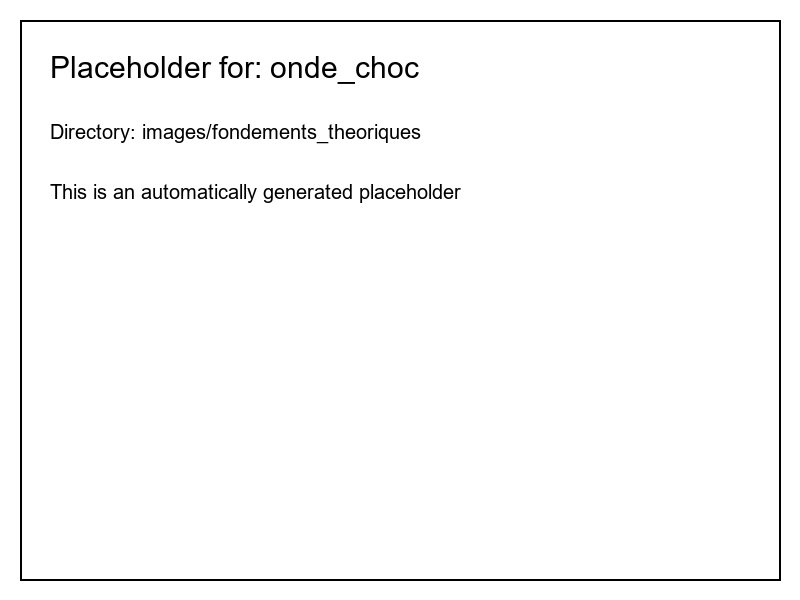
\includegraphics[width=0.8\textwidth]{images/fondements_theoriques/onde_choc}
\caption{Propagation d'une onde de choc : (a) représentation dans le plan $(x,t)$; (b) représentation sur le diagramme fondamental.}
\label{fig:onde_choc}
\end{figure}

\subsection{Problème de Riemann}
\label{subsec:riemann}

Le **problème de Riemann**, fondamental pour la résolution numérique de l'équation de conservation, consiste à déterminer l'évolution temporelle d'une discontinuité initiale. Il permet d'analyser comment des conditions initiales discontinues se résolvent en ondes de choc ou de raréfaction, fournissant ainsi une base pour comprendre des phénomènes de trafic complexes.

\begin{definition}[Problème de Riemann]
Le problème de Riemann pour l'équation de conservation du trafic consiste à résoudre :
\begin{align}
\pd{\dens}{t} + \pd{\flow(\dens)}{x} &= 0\\
\dens(x,0) &= 
\begin{cases}
\dens_L, & x < 0\\
\dens_R, & x > 0
\end{cases}
\end{align}
où $\dens_L$ et $\dens_R$ sont des constantes représentant les densités à gauche et à droite de la discontinuité initiale, respectivement.
\end{definition}

La solution du problème de Riemann dépend de la position relative des états $\dens_L$ et $\dens_R$ par rapport à la densité critique $\dens_c$ :

\begin{enumerate}
    \item Si $\dens_L < \dens_R < \dens_c$ ou $\dens_c < \dens_L < \dens_R$ : formation d'une **onde de choc**. Une onde de choc se forme lorsqu'une densité plus élevée rattrape une densité plus faible, créant une transition abrupte.
    \item Si $\dens_R < \dens_L < \dens_c$ ou $\dens_c < \dens_R < \dens_L$ : formation d'une **onde de raréfaction**. Une onde de raréfaction se forme lorsqu'une densité plus faible suit une densité plus élevée, créant une transition progressive.
    \item Si $\dens_L < \dens_c < \dens_R$ : formation d'une **onde de choc de congestion** (apparition d'un embouteillage). Dans ce cas, la densité à droite est suffisamment élevée pour provoquer une congestion qui se propage vers l'amont.
    \item Si $\dens_R < \dens_c < \dens_L$ : formation d'une **onde de raréfaction** (dissipation d'un embouteillage). Ici, la différence de densité favorise la dissipation de la congestion.
\end{enumerate}

Le modèle de Lighthill-Whitham-Richards (LWR) prédit que les véhicules passant à travers une zone de concentration accrue devront réduire leur vitesse de manière abrupte à l'entrée, créant une onde de choc. En revanche, ils pourront augmenter leur vitesse progressivement en sortant de cette zone.

Il convient de noter que d'autres modèles dits du second ordre peuvent tenir compte de l'accélération des conducteurs, offrant ainsi une représentation plus réaliste des transitions de vitesse, mais au prix d'une complexité mathématique accrue.

En pratique, les conditions initiales sont rarement aussi simples que celles du problème de Riemann, mais la compréhension de ses solutions est essentielle pour la conception d'algorithmes numériques robustes et précis.

\section{Limites du Modèle LWR Standard}
\label{sec:limites_lwr}

Malgré sa simplicité et son efficacité pour décrire les phénomènes macroscopiques du trafic, le modèle LWR standard présente plusieurs limitations qui rendent nécessaire son extension, particulièrement dans le contexte béninois :

\subsection{Homogénéité des Véhicules}
\label{subsec:homogeneite}

Le modèle LWR suppose que tous les véhicules sont identiques, ce qui ne reflète pas la réalité du trafic routier, et particulièrement pas celle du Bénin où cohabitent voitures, motos, camions, et autres types de véhicules.

\begin{remark}
Au Bénin, les motos représentent plus de 70\% du parc automobile, créant une dynamique de trafic très différente de celle modélisée par le LWR standard.
\end{remark}

\subsection{Relation Vitesse-Densité Unique}
\label{subsec:relation_unique}

Le modèle utilise une relation vitesse-densité unique pour tous les véhicules, ne tenant pas compte des différences de comportement entre classes de véhicules, ni de l'impact du type de revêtement routier sur la vitesse.

\subsection{Absence d'Interactions Complexes}
\label{subsec:interactions}

Le LWR ne modélise pas les interactions complexes entre différentes classes de véhicules, comme le comportement gap-filling des motos qui peuvent s'infiltrer entre les voitures.

\subsection{Modélisation Limitée des Intersections}
\label{subsec:intersections}

Le traitement des intersections et points singuliers du réseau n'est pas intégré de manière satisfaisante dans le modèle standard, alors qu'ils constituent des points critiques de la circulation urbaine au Bénin.

\section{Extensions Existantes du Modèle LWR}
\label{sec:extensions_existantes}

Différentes extensions du modèle LWR ont été proposées dans la littérature pour répondre à certaines de ses limitations :

\subsection{Modèles Multiclasses}
\label{subsec:multiclasses}

Les modèles multiclasses, comme ceux proposés par Wong et Wong \cite{wong2002multi}, étendent le LWR pour tenir compte de différentes classes de véhicules avec leurs propres caractéristiques (vitesse maximale, taille).

\begin{example}[Modèle de Wong et Wong]
Ce modèle propose un système d'équations couplées :
\begin{align}
\pd{\densi{i}}{t} + \pd{\flowi{i}}{x} &= 0, \quad \forall i \in \{1,\ldots,N\}\\
\veli{i} &= \veli{i}\left(\sum_{j=1}^{N} \densi{j}\right)
\end{align}
où les fonctions $\veli{i}$ tiennent compte de la densité totale.
\end{example}

\subsection{Modèles à Effets Non-locaux}
\label{subsec:non_local}

Ces modèles, comme celui de Zhang \cite{zhang2003non}, prennent en compte l'anticipation des conducteurs en intégrant une dépendance non-locale de la vitesse.

\subsection{Modèles de Transmission Cellulaire}
\label{subsec:cell_transmission}

Le modèle de transmission cellulaire de Daganzo \cite{daganzo1995cell} est une discrétisation du LWR qui facilite la modélisation des intersections et des réseaux complexes.

\section{Illustration Numérique du Modèle LWR}
\label{sec:illustration_numerique}

Pour compléter notre étude théorique et visualiser concrètement les phénomènes décrits précédemment (ondes de choc, raréfactions), nous avons implémenté une résolution numérique du modèle LWR. Les simulations présentées ci-dessous utilisent le schéma de Godunov, choisi pour sa capacité à préserver la nature conservative de l'équation et sa robustesse face aux discontinuités inhérentes aux problèmes de trafic. Contrairement à d'autres méthodes numériques, ce schéma évite l'apparition d'oscillations non physiques au voisinage des chocs tout en maintenant une précision satisfaisante. Les fondements mathématiques et détails d'implémentation de cette méthode sont présentés dans l'Annexe.
\subsection{Schéma Numérique de Godunov}
\label{subsec:godunov}

Pour résoudre numériquement l'équation de conservation \eqref{eq:conservation_lwr}, nous discrétisons le domaine spatial en cellules de longueur $\Delta x$ et le temps en pas $\Delta t$. Le schéma de Godunov \cite{godunov1959finite,leveque1992numerical} se présente alors sous la forme :

\begin{equation}
\rho_i^{n+1} = \rho_i^n - \frac{\Delta t}{\Delta x}(F_{i+\frac{1}{2}}^n - F_{i-\frac{1}{2}}^n)
\end{equation}

où $\rho_i^n$ représente la densité moyenne dans la cellule $i$ au temps $n$\Delta$ t$, et $F_{i\pm\frac{1}{2}}^n$ sont les flux numériques aux interfaces. Ces flux sont déterminés en résolvant localement un problème de Riemann :

\begin{equation}
F_{i+\frac{1}{2}} = \mathcal{F}(\rho_i^n, \rho_{i+1}^n)
\end{equation}
    
Nous avons choisi ce schéma numérique car il est particulièrement adapté aux lois de conservation hyperboliques et permet de capturer précisément les discontinuités (ondes de choc) sans introduire d'oscillations parasites \cite{toro2013riemann}. Les détails complets concernant l'implémentation du schéma, les calculs des flux numériques et les preuves de convergence sont présentés dans l'Annexe \ref{annex:schemas_numeriques}.
    
\subsection{Scénarios de Simulation}
\label{subsec:scenarios}

Nous présentons ici trois scénarios caractéristiques qui illustrent les phénomènes fondamentaux du trafic routier modélisés par le LWR :

\begin{enumerate}
    \item \textbf{Feu rouge} : formation d'une congestion en amont d'un feu rouge et sa dissipation après le passage au vert.
    \item \textbf{Onde de choc} : rencontre d'un trafic rapide et d'un trafic lent créant une onde de choc se propageant en amont.
    \item \textbf{Onde de raréfaction} : accélération progressive d'un trafic initialement congestionné.
\end{enumerate}

\subsubsection{Feu Rouge}
\label{subsubsec:feu_rouge}

Considérons une route de 10 km où le trafic circule initialement à densité modérée ($\rho = 0,2$\rho$_{\max}$), mais avec un arrêt complet (densité proche de $\rho_{\max}$) au niveau d'un feu rouge situé à 5 km du début de la route. La Figure \ref{fig:feu_rouge} illustre l'évolution spatio-temporelle de la densité, de la vitesse et du flux après le passage du feu au vert.

\begin{figure}[htbp]
\centering
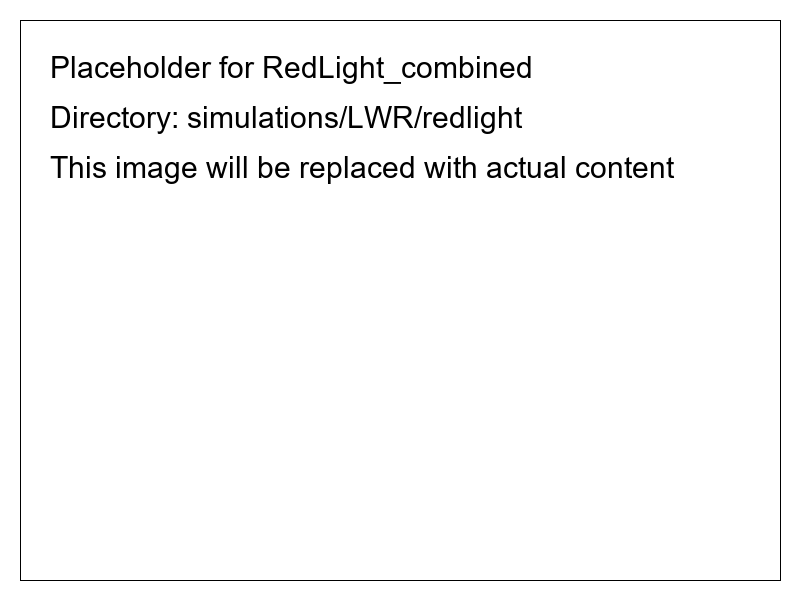
\includegraphics[width=1.0\textwidth]{simulations/LWR/redlight/RedLight_combined}
\caption{Simulation de la dissipation d'un embouteillage après le passage d'un feu au vert. De haut en bas : (a) Évolution de la densité, (b) Évolution de la vitesse, (c) Évolution du flux.}
\label{fig:feu_rouge}
\end{figure}

On observe clairement la formation d'une onde de choc qui se propage en amont du feu lorsque celui-ci est rouge, puis une onde de raréfaction qui se développe après le passage au vert. La vitesse de propagation de l'onde de choc correspond à la pente de la tangente au diagramme fondamental entre les états de trafic de part et d'autre du choc, comme prédit par la théorie.

\subsubsection{Onde de Choc}
\label{subsubsec:onde_choc_sim}

Dans ce scénario, nous simulons une route de 20 km avec un trafic fluide ($\rho = 0,1$\rho$_{\max}$) en amont et un trafic dense ($\rho = 0,7$\rho$_{\max}$) en aval. La Figure \ref{fig:sim_onde_choc} montre la formation et la propagation d'une onde de choc à l'interface entre ces deux régimes.

\begin{figure}[htbp]
\centering
\includegraphics[width=1.0\textwidth]{simulations/LWR/shock/ShockWave_combined}
\caption{Simulation de la formation et propagation d'une onde de choc. De haut en bas : (a) Évolution de la densité, (b) Évolution de la vitesse, (c) Évolution du flux.}
\label{fig:sim_onde_choc}
\end{figure}


On observe que l'onde de choc se propage en amont avec une vitesse négative constante, conformément à la théorie. Les véhicules doivent ralentir brusquement en atteignant le front de l'onde, ce qui correspond à une discontinuité dans le profil de vitesse.

\subsubsection{Onde de Raréfaction}
\label{subsubsec:rarefaction_sim}

Ce scénario illustre la dissipation progressive d'un embouteillage, représentée par une onde de raréfaction. Nous considérons une route de 20 km avec un trafic dense ($\rho = 0,7$\rho$_{\max}$) en amont et un trafic fluide ($\rho = 0,1$\rho$_{\max}$) en aval. La Figure \ref{fig:sim_rarefaction} montre l'évolution de cette situation.

\begin{figure}[htbp]
\centering
\includegraphics[width=1.0\textwidth]{simulations/LWR/rarefaction/RarefactionWave_combined}
\caption{Simulation d'une onde de raréfaction. De haut en bas : (a) Évolution de la densité, (b) Évolution de la vitesse, (c) Évolution du flux.}
\label{fig:sim_rarefaction}
\end{figure}

Contrairement à l'onde de choc, la transition est progressive : les véhicules accélèrent graduellement en sortant de la zone congestionnée, créant un éventail de caractéristiques dans le plan espace-temps.

\subsection{Limitations Révélées par les Simulations}
\label{subsec:limitations_sim}

Ces simulations, bien qu'illustrant correctement certains phénomènes de trafic, mettent en évidence plusieurs limitations du modèle LWR standard face aux spécificités du contexte béninois :

\begin{itemize}
    \item \textbf{Homogénéité des véhicules} : Les simulations supposent un flux homogène de véhicules identiques, ce qui ne reflète pas la diversité du parc automobile béninois dominé par les motos (zémidjans). La Figure \ref{fig:comparaison_flux} montre la différence entre un flux simulé homogène et des observations réelles à Cotonou, où la présence de motos crée des comportements de trafic distincts.
    
    \item \textbf{Comportement aux intersections} : Le modèle LWR standard ne peut pas simuler correctement les comportements spécifiques aux intersections non régulées fréquentes dans les villes béninoises, où les motos s'infiltrent entre les voitures et ne respectent pas nécessairement les files d'attente traditionnelles.
    
    \item \textbf{Effets de l'état des routes} : Les simulations ne tiennent pas compte de l'état variable des infrastructures routières, un facteur crucial au Bénin où la qualité du revêtement influe significativement sur les vitesses pratiquées.
\end{itemize}

% Ces limitations, mises en évidence par la confrontation des simulations avec les observations de terrain, justifient pleinement la nécessité de développer une extension du modèle LWR adaptée aux spécificités du trafic routier béninois. Les fondements mathématiques rigoureux et les démonstrations formelles qui sous-tendent cette extension sont détaillés dans l'Annexe \ref{annexe:demonstrations}.

% \begin{figure}[htbp]
% \centering
% 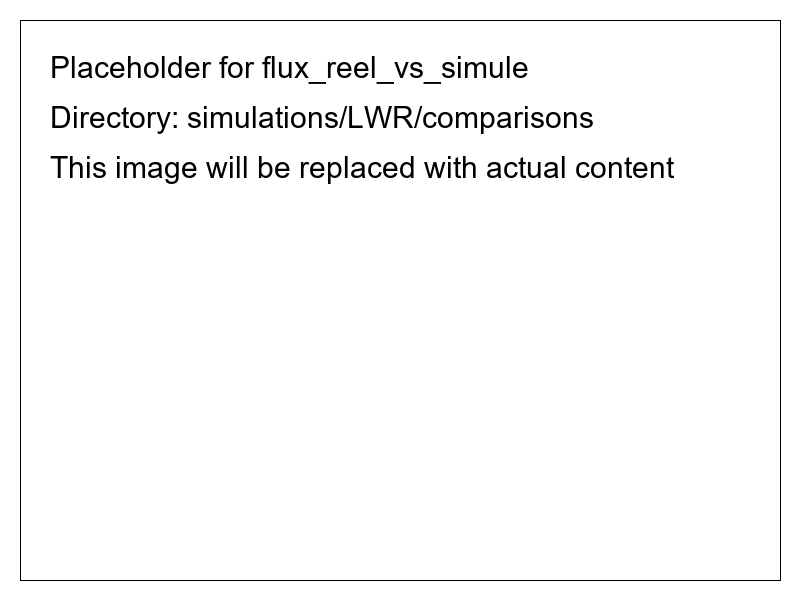
\includegraphics[width=0.8\textwidth]{simulations/LWR/comparisons/flux_reel_vs_simule}
% \caption{Comparaison entre le flux simulé par le modèle LWR standard et des observations réelles dans une rue typique de Cotonou. Les différences significatives soulignent la nécessité d'adapter le modèle au contexte béninois.}
% \label{fig:comparaison_flux}
% \end{figure}

\section{Vers une Extension Adaptée au Contexte Béninois}
\label{sec:vers_extension}

L'extension que nous proposons vise à adapter le modèle LWR au contexte béninois en combinant et enrichissant plusieurs approches existantes :

\begin{itemize}
\item Adoption d'un cadre multiclasses pour distinguer les différents types de véhicules;
\item Introduction d'un coefficient de ralentissement lié au type de revêtement;
\item Développement de fonctions de modulation spécifiques pour les motos;
\item Traitement particulier des intersections et points singuliers.
\end{itemize}

Ces adaptations seront détaillées dans le Chapitre \ref{chap:extension_modele}, après une analyse approfondie des spécificités du réseau routier béninois et du rôle des motos dans le Chapitre \ref{chap:specificites_benin}.

\chapter{Spécificités du Réseau Routier Béninois et Rôle des Motos}
\label{chap:specificites_benin}

\section{Diversité des Infrastructures au Bénin}
\label{sec:diversite_infrastructures}

Le réseau routier béninois présente une grande hétérogénéité qui impacte significativement la dynamique du trafic. Cette diversité se manifeste à plusieurs niveaux : qualité du revêtement, largeur des voies, présence ou absence de trottoirs, et organisation des intersections.

\subsection{Types de Revêtement et État des Routes}
\label{subsec:types_revetement}

Selon les données de la Banque Mondiale \cite{worldbank2019benin}, le réseau routier béninois totalise environ 18 500 km, dont seulement 9,7\% (1 800 km) sont pavés à l'échelle nationale. Cette proportion varie significativement entre les zones rurales et urbaines. Le réseau comprend quatre principales catégories de revêtement, chacune influençant différemment la circulation des véhicules :

\begin{itemize}
\item \textbf{Routes bitumées} : Principalement présentes dans les grandes villes et sur les axes interurbains majeurs, elles peuvent représenter jusqu'à 30-35\% du réseau urbain dans des villes comme Cotonou. Leur qualité varie considérablement, allant de voies rapides bien entretenues à des routes fortement dégradées avec nids-de-poule.

\item \textbf{Routes en terre} : Constituant la majorité du réseau national, ces routes non revêtues sont particulièrement sensibles aux conditions climatiques. En saison sèche, elles génèrent de la poussière affectant la visibilité, tandis qu'en saison des pluies, elles deviennent souvent boueuses et difficilement praticables pour les voitures, mais restent accessibles aux motos.

\item \textbf{Routes pavées} : Présentes dans certaines zones urbaines et périurbaines, ces routes offrent une bonne adhérence mais créent des vibrations qui ralentissent les véhicules, particulièrement les voitures, alors que les motos y maintiennent une vitesse plus élevée.

\item \textbf{Pistes et voies informelles} : Ces chemins, souvent créés par l'usage répété, sont généralement inaccessibles aux voitures mais fréquemment empruntés par les motos, créant un réseau parallèle non officiel.
\end{itemize}

\begin{figure}[htbp]
\centering
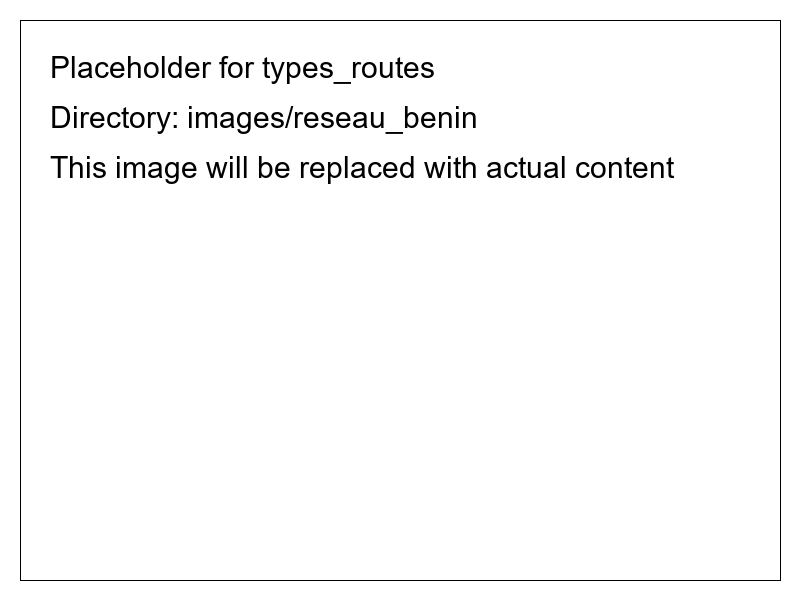
\includegraphics[width=0.9\textwidth]{images/reseau_benin/types_routes}
\caption{Les différents types de routes au Bénin : (a) route bitumée à Cotonou; (b) route en terre en zone périurbaine; (c) route pavée; (d) piste accessible uniquement aux motos.}
\label{fig:types_routes}
\end{figure}

\begin{remark}
Cette diversité des revêtements routiers affecte différemment chaque classe de véhicule, les motos étant généralement moins impactées par la dégradation du revêtement que les voitures, ce qui nécessitera une prise en compte spécifique dans notre modélisation.
\end{remark}

\subsection{Organisation Spatiale du Réseau}
\label{subsec:organisation_spatiale}

La configuration du réseau routier béninois présente plusieurs particularités structurelles :

\begin{itemize}
\item \textbf{Structure radiale} dans les grandes villes comme Cotonou, avec des axes principaux convergeant vers le centre, créant des points de congestion.

\item \textbf{Voies à largeur variable} : La largeur des routes change fréquemment, créant des goulots d'étranglement où s'accumulent les véhicules. Ces variations affectent différemment les classes de véhicules, les motos étant moins impactées.

\item \textbf{Rareté des voies rapides dédiées} : Le réseau compte peu d'autoroutes ou voies rapides dédiées, ce qui limite la séparation des flux de véhicules selon leur vitesse.

\item \textbf{Zones d'habitat spontané} créant des réseaux irréguliers où coexistent véhicules et piétons, avec une forte présence de motos.
\end{itemize}

\subsection{Gestion des Intersections}
\label{subsec:gestion_intersections}

Les intersections au Bénin présentent des spécificités qui complexifient leur modélisation :

\begin{itemize}
\item \textbf{Faible présence de feux de circulation} : Moins de 20\% des intersections urbaines sont régulées par des feux, souvent sujets à des pannes. Cette situation est caractéristique de nombreuses villes d'Afrique subsaharienne \cite{loggoh2019traffic}.

\item \textbf{Ronds-points surchargés} : Les ronds-points, nombreux dans les villes, deviennent des points de congestion majeurs aux heures de pointe.

\item \textbf{Prédominance de la priorité à droite} ou de la négociation informelle entre conducteurs.

\item \textbf{Présence d'agents de circulation} aux intersections majeures, introduisant une variabilité humaine dans la régulation.
\end{itemize}

\begin{figure}[htbp]
\centering
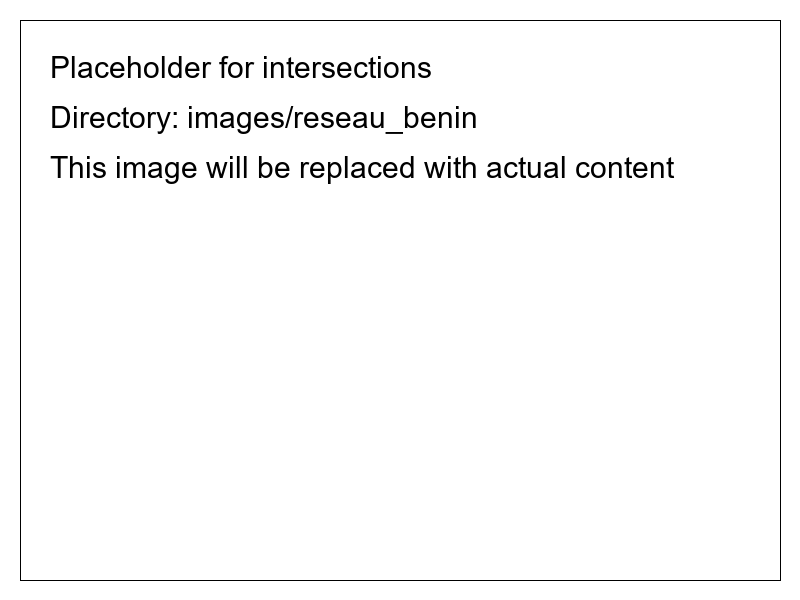
\includegraphics[width=0.8\textwidth]{images/reseau_benin/intersections}
\caption{Gestion des intersections au Bénin : (a) carrefour sans feux avec agent de circulation; (b) rond-point congestionné; (c) intersection non régulée avec motos prédominantes.}
\label{fig:intersections}
\end{figure}

\begin{theorem}[Modélisation des intersections béninoises]
Dans notre modèle, une intersection sera représentée par un terme source/puits $S_i(x,t)$ dans l'équation de conservation, avec :
\begin{align}
S_i(x,t) = \alpha_i(t) \cdot \delta(x-x_0)
\end{align}
où $\alpha_i(t)$ représente le flux entrant/sortant de véhicules de classe $i$, $\delta$ est la distribution de Dirac, et $x_0$ la position de l'intersection.
\end{theorem}

\section{Collecte et Exploitation des Données Béninoises}
\label{sec:collecte_donnees}

La modélisation précise du trafic béninois nécessite des données spécifiques au contexte local.

\subsection{Méthodologie de Collecte des Données}
\label{subsec:methodologie_collecte}

En raison de limitations pratiques et logistiques, notre approche de collecte de données s'appuie principalement sur les sources suivantes :

\begin{itemize}
\item \textbf{Données de Google Maps Traffic Layer} : Cette source constitue notre outil principal, fournissant des informations en temps réel sur la congestion et les vitesses moyennes sur différents axes routiers. L'API de Google Maps permet d'extraire des données historiques de trafic à différentes heures de la journée et jours de la semaine, offrant une vision dynamique des conditions de circulation. Nous utilisons ces données pour :
  \begin{itemize}
    \item Identifier les zones de congestion récurrentes
    \item Estimer les vitesses moyennes sur différents types de routes
    \item Observer les variations temporelles (heures de pointe, différences jour/nuit, jours ouvrables/week-end)
    \item Évaluer l'impact des conditions météorologiques sur le trafic
  \end{itemize}

\item \textbf{Données statistiques officielles} du Ministère des Transports du Bénin et de l'Institut National de la Statistique et de l'Analyse Économique (INSAE), notamment pour la composition du parc automobile et la répartition des types de véhicules.

\item \textbf{Littérature existante et études antérieures}, particulièrement les travaux de \cite{loggoh2019traffic} et \cite{aerc2019taxi}, qui fournissent des informations précieuses sur les comportements de conduite et les spécificités du trafic béninois.

\item \textbf{Observations qualitatives} documentées sous forme de photographies et notes descriptives lors de visites sur le terrain, sans mesures quantitatives systématiques.

\item \textbf{Consultation d'experts locaux} et de professionnels du transport, notamment des urbanistes, des ingénieurs en transport et des responsables de la sécurité routière, qui ont partagé leurs connaissances et expériences.
\end{itemize}

\begin{remark}
Bien que cette approche présente des limitations, notamment l'absence de données détaillées sur la composition exacte du trafic et les comportements spécifiques des différentes classes de véhicules, elle permet néanmoins d'obtenir une vision globale des dynamiques de circulation au Bénin.
\end{remark}

\subsection{Traitement et Analyse des Données}
\label{subsec:traitement_donnees}

Malgré les limitations dans la collecte, nous avons développé une méthodologie adaptée pour exploiter au mieux les données disponibles :

\begin{enumerate}
\item \textbf{Extraction systématique des données de Google Maps} à intervalles réguliers (toutes les heures pendant plusieurs semaines) pour constituer une base temporelle représentative.

\item \textbf{Classification des segments routiers} selon leur type (bitumé, terre, pavé) basée sur les données cartographiques et les observations qualitatives.

\item \textbf{Analyse des variations temporelles} pour identifier les motifs récurrents de congestion et estimer les densités relatives de trafic.

\item \textbf{Croisement avec les données statistiques officielles} pour inférer la composition probable du trafic dans différentes zones et à différentes périodes.

\item \textbf{Validation par triangulation} avec les observations qualitatives et les informations issues de la littérature existante.
\end{enumerate}

\section{Spécificités des Types de Véhicules et Place des Motos}
\label{sec:specificites_vehicules}

\subsection{Hétérogénéité du Parc Automobile}
\label{subsec:heterogeneite_parc}

Le parc automobile béninois présente une grande diversité qui impacte la dynamique du trafic. Selon les études disponibles, notamment celle de l'AERC \cite{aerc2019taxi}, la composition du trafic se caractérise par :

\begin{itemize}
\item \textbf{Motos et motocyclettes} (localement appelées "Zémidjans" lorsqu'elles servent de taxi) : Représentant plus de 70\% des véhicules en circulation, elles constituent l'épine dorsale du transport urbain \cite{aerc2019taxi}.

\item \textbf{Voitures particulières} : Environ 15\% du parc, composé de véhicules d'âges et de tailles variés, souvent importés d'occasion.

\item \textbf{Taxis-ville} (généralement des berlines peintes en jaune) : Environ 5\% du parc dans les zones urbaines.

\item \textbf{Minibus et bus} : Services de transport en commun, représentant 3\% des véhicules.

\item \textbf{Camions et poids lourds} : Environ 7\% des véhicules, principalement sur les axes interurbains et les zones portuaires.
\end{itemize}

Cette hétérogénéité se traduit par des différences significatives dans les paramètres de conduite, comme illustré dans le tableau suivant :

\begin{table}[htbp]
\centering
\caption{Paramètres caractéristiques par classe de véhicule}
\label{tab:parametres_vehicules}
\begin{tabular}{lcccc}
\toprule
\textbf{Classe} & \textbf{$v_{i,\max}^0$ (km/h)} & \textbf{$\rho_{i,\max}$ (véh/km)} & \textbf{Coefficient $\mu_i$} & \textbf{Impact relatif} \\
 & & & & \textbf{du type de route} \\
\midrule
Motos & 60 & 240 & -- & 1.0 \\
Voitures & 70 & 180 & 0.3 & 0.7 \\
Taxis & 65 & 180 & 0.4 & 0.8 \\
Bus & 55 & 140 & 0.5 & 0.6 \\
Camions & 50 & 120 & 0.6 & 0.5 \\
\bottomrule
\end{tabular}
\end{table}

\subsection{Rôle Prépondérant des Motos dans le Trafic Béninois}
\label{subsec:role_motos}

Les motos jouent un rôle central dans le trafic béninois qui les distingue fondamentalement des autres classes de véhicules. Les études comme celles de \cite{loggoh2019traffic} et \cite{aerc2019taxi} confirment leur prédominance et leurs comportements spécifiques :

\begin{itemize}
\item \textbf{Capacité d'infiltration} : Les motos peuvent s'insérer dans des espaces réduits entre les voitures, créant un flux qui s'écoule même en situation apparemment congestionnée \cite{kumar2018motorcycle}.

\item \textbf{Trajectoires flexibles} : Contrairement aux voitures confinées à leurs voies, les motos suivent des trajectoires opportunistes, changeant fréquemment de direction.

\item \textbf{Comportement collectif} : Les motos tendent à se regrouper aux feux rouges et intersections, formant des "essaims" qui démarrent rapidement au feu vert.

\item \textbf{Adaptation aux infrastructures dégradées} : Les motos peuvent maintenir une vitesse relativement élevée sur des surfaces où les voitures doivent considérablement ralentir \cite{karthik2019estimation}.
\end{itemize}

\begin{definition}[Gap-filling]
Le comportement gap-filling désigne la capacité des motos à occuper les espaces entre les véhicules plus grands, augmentant ainsi la densité effective du trafic sans nécessairement réduire les vitesses \cite{fan2013heterogeneous}.
\end{definition}

\begin{definition}[Interweaving]
Le comportement interweaving désigne le mouvement en zigzag des motos entre les files de véhicules, créant un flux transversal qui peut perturber l'écoulement des autres classes \cite{kumar2018motorcycle}.
\end{definition}

Ces comportements spécifiques nécessitent une modélisation dédiée dans notre extension du modèle LWR, notamment à travers des fonctions de modulation qui seront introduites dans le chapitre suivant.

\begin{figure}[htbp]
\centering
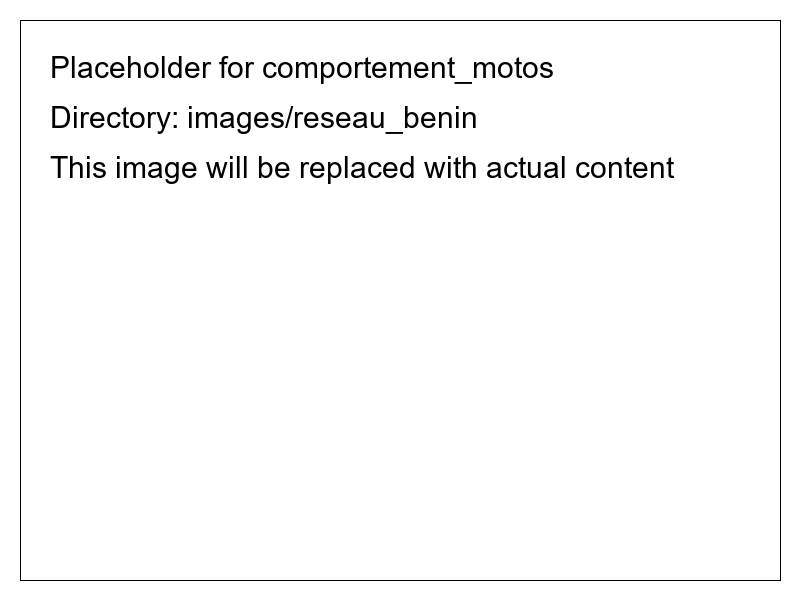
\includegraphics[width=0.9\textwidth]{images/reseau_benin/comportement_motos}
\caption{Comportements spécifiques des motos dans le trafic béninois : (a) gap-filling entre voitures; (b) regroupement aux intersections; (c) trajectoires flexibles contournant les obstacles.}
\label{fig:comportement_motos}
\end{figure}

\subsection{Impact des Motos sur la Dynamique Globale du Trafic}
\label{subsec:impact_motos}

La prédominance des motos modifie profondément la dynamique du trafic par rapport aux modèles classiques. Les études de \cite{wong2002multi} et \cite{fan2013heterogeneous} ont démontré plusieurs impacts significatifs :

\begin{itemize}
\item \textbf{Augmentation de la capacité effective} des routes : En utilisant l'espace disponible de manière plus efficace, les motos permettent d'accroître le flux total de véhicules \cite{chanut2005modeles}.

\item \textbf{Modification des relations vitesse-densité} : La présence de nombreuses motos peut maintenir des vitesses moyennes relativement élevées même à forte densité totale, contrairement au modèle classique de Greenshields \cite{greenshields1935study}.

\item \textbf{Transformation des intersections} en points de mélange complexe où les principes habituels de priorité sont souvent remplacés par une négociation constante entre usagers \cite{akcelik2003relationship}.

\item \textbf{Création de réseaux parallèles informels} : Les motos empruntent souvent des chemins inaccessibles aux autres véhicules, redistribuant le trafic de manière difficile à prédire avec les modèles classiques.
\end{itemize}

\begin{proposition}
Dans un flux mixte avec une proportion significative de motos, la relation entre la densité totale $\rho$ et le flux total $q$ n'est plus une fonction simple comme dans le modèle de Greenshields \cite{greenshields1935study}, mais dépend de la composition du trafic :
\begin{align}
q(\rho, \rho_M) = \sum_{i=1}^N \rho_i \cdot v_i(\rho, \rho_M)
\end{align}
où $\rho_M$ est la densité des motos, et les fonctions $v_i$ intègrent l'effet des motos sur chaque classe.
\end{proposition}

\section{Vers un Modèle Adapté aux Spécificités Béninoises}
\label{sec:vers_modele_adapte}

Les spécificités du réseau routier béninois et le rôle particulier des motos nécessitent une adaptation profonde des modèles de trafic standards comme le modèle LWR \cite{lighthill1955kinematic, richards1956shock}.

\begin{itemize}
\item La \textbf{diversité des infrastructures} exige l'introduction de facteurs spécifiques à chaque type de route et classe de véhicule dans notre modèle.

\item L'\textbf{hétérogénéité du parc automobile} justifie une approche multiclasses avec des paramètres distincts pour chaque type de véhicule, comme proposé par \cite{wong2002multi}.

\item Le \textbf{comportement spécifique des motos} requiert des fonctions de modulation traduisant leur impact sur les autres classes de véhicules, s'inspirant des approches de \cite{zhang2003non}.

\item La \textbf{gestion particulière des intersections} nécessite un traitement mathématique adapté des conditions aux limites et des termes sources/puits, comme suggéré par \cite{daganzo1995cell}.
\end{itemize}

Dans le chapitre suivant, nous développerons un cadre mathématique intégrant ces spécificités dans une extension du modèle LWR qui représentera fidèlement la dynamique du trafic routier au Bénin.

% !TEX root = ../memoire.tex
\chapter{Extension du Modèle LWR et Modélisation Spécifique des Motos}\label{chap:extension_modele}

\section{Introduction et Motivation}\label{sec:intro_motivation}

Comme nous l'avons démontré dans les chapitres précédents, le modèle LWR standard présente des limitations importantes lorsqu'il est confronté aux réalités du trafic routier béninois. Dans ce chapitre, nous proposons une extension progressive du modèle LWR pour répondre spécifiquement à ces défis.

Rappelons que le modèle LWR standard repose sur l'équation de conservation:
\begin{equation}
\frac{\partial \rho}{\partial t} + \frac{\partial(\rho v)}{\partial x} = 0
\end{equation}
avec la relation constitutive de Greenshields:
\begin{equation}
v(\rho) = v_{\max}\left(1 - \frac{\rho}{\rho_{\max}}\right)
\end{equation}

Notre extension s'articule autour de trois innovations principales:
\begin{enumerate}
\item L'adoption d'une approche multiclasse pour distinguer les différents types de véhicules
\item L'introduction d'un coefficient de ralentissement lié au revêtement routier
\item Le développement de fonctions de modulation spécifiques pour modéliser le comportement des motos
\end{enumerate}

\section{Extension Multiclasse du Modèle LWR}\label{sec:extension_multiclasse}

\subsection{Motivation de l'Approche Multiclasse}\label{subsec:motivation_multiclasse}

La première limitation majeure du modèle LWR standard est l'hypothèse d'homogénéité des véhicules. Au Bénin, comme nous l'avons observé au Chapitre \ref{chap:specificites_benin}, le trafic se caractérise par une grande diversité de véhicules, avec une prédominance des motos (plus de 70\% du parc automobile).

L'approche multiclasse permet de remédier à cette limitation en distinguant explicitement différentes classes de véhicules, chacune avec ses propres caractéristiques. Cette approche a été initialement proposée par Wong et Wong \cite{wong2002multi} et adaptée par d'autres chercheurs \cite{zhang2003non, loggoh2019traffic}.

\subsection{Système d'Équations de Conservation par Classe}\label{subsec:systeme_equations}

Dans notre extension multiclasse du modèle LWR, nous considérons $N$ classes de véhicules (motos, voitures, taxis, bus, camions, etc.). Pour chaque classe $i \in \{1,...,N\}$, nous définissons:

\begin{itemize}
\item $\rho_i(x,t)$ : densité de la classe $i$ [véh/km]
\item $v_i(x,t)$ : vitesse moyenne de la classe $i$ [km/h]
\item $q_i(x,t) = \rho_i(x,t) \cdot v_i(x,t)$ : flux de la classe $i$ [véh/h]
\end{itemize}

En appliquant le principe de conservation de la masse à chaque classe, nous obtenons un système de $N$ équations:

\begin{empheq}[box=\colorbox{lightblue!15}]{align}
\frac{\partial \rho_i}{\partial t} + \frac{\partial(\rho_i v_i)}{\partial x} = S_i(x,t), \quad i \in \{1,...,N\}
\label{eq:conservation_multiclasse}
\end{empheq}

où $S_i(x,t)$ représente un terme source/puits pour la classe $i$ (entrées/sorties à une intersection, changements de classe, etc.).

La densité totale du trafic est simplement la somme des densités de chaque classe:
\begin{equation}
\rho(x,t) = \sum_{i=1}^N \rho_i(x,t)
\label{eq:densite_totale}
\end{equation}

\subsection{Relations Constitutives Multiclasses}\label{subsec:relations_constitutives}

À ce stade, nous devons définir comment la vitesse de chaque classe $v_i$ dépend des densités. Une approche simple consisterait à étendre directement la relation de Greenshields à chaque classe:

\begin{equation}
v_i(\rho) = v_{i,0}\left(1 - \frac{\rho}{\rho_{\max}}\right)
\label{eq:vitesse_multiclasse_simple}
\end{equation}

où $v_{i,0}$ est la vitesse libre de référence pour la classe $i$ et $\rho_{\max}$ est la densité maximale commune.

Cependant, cette formulation simple ne capture pas toutes les particularités du trafic béninois. Nous allons progressivement enrichir cette relation dans les sections suivantes.

\section{Intégration de l'Effet du Revêtement Routier}
\label{sec:effet_revetement}

\subsection{Problématique du Revêtement au Bénin}
\label{subsec:problematique_revetement}

Comme détaillé au Chapitre \ref{chap:specificites_benin}, le réseau routier béninois se caractérise par une grande diversité de revêtements (bitume en bon état, bitume dégradé, terre compactée, pavés), avec des impacts variables selon les types de véhicules. Le modèle LWR standard et même son extension multiclasse simple ne tiennent pas compte de cette hétérogénéité spatiale.

\subsection{Coefficient de Ralentissement Dépendant de la Position}
\label{subsec:coefficient_ralentissement}

Pour intégrer l'effet du revêtement routier, nous introduisons un coefficient de ralentissement $\lambda_i(x) \in [0,1]$ qui module la vitesse libre de référence pour chaque classe de véhicule:

\begin{empheq}[box=\colorbox{lightblue!15}]{align}
v_i(\rho, x) = \lambda_i(x) \cdot v_{i,0} \cdot \left(1 - \frac{\rho}{\rho_{\max}}\right)
\label{eq:vitesse_avec_revetement}
\end{empheq}

Ce coefficient présente les propriétés suivantes:
\begin{itemize}
\item $\lambda_i(x) = 1$ pour un revêtement parfait (route bitumée neuve)
\item $\lambda_i(x) \rightarrow 0$ quand la qualité du revêtement se dégrade fortement
\item $\lambda_M(x) > \lambda_i(x)$ pour $i \neq M$ sur des revêtements dégradés (les motos sont moins affectées par la mauvaise qualité des routes)
\end{itemize}

Le Tableau \ref{tab:valeurs_lambda} présente des valeurs typiques de ce coefficient selon le type de revêtement et la classe de véhicule, dérivées de nos observations sur le terrain.

\begin{table}[htbp]
\centering
\caption{Valeurs typiques du coefficient $\lambda_i(x)$ par classe de véhicule et type de route}
\label{tab:valeurs_lambda}
\begin{tabular}{lccccc}
\toprule
\textbf{Type de revêtement} & \textbf{Motos} & \textbf{Voitures} & \textbf{Taxis} & \textbf{Bus} & \textbf{Camions} \\
\midrule
Bitume (bon état) & 0.95-1.00 & 0.90-0.95 & 0.88-0.93 & 0.85-0.90 & 0.80-0.90 \\
Bitume (dégradé) & 0.75-0.85 & 0.60-0.75 & 0.65-0.75 & 0.60-0.70 & 0.55-0.65 \\
Terre compactée & 0.70-0.80 & 0.45-0.60 & 0.50-0.60 & 0.40-0.55 & 0.35-0.50 \\
Pavé & 0.75-0.85 & 0.55-0.65 & 0.60-0.70 & 0.50-0.65 & 0.50-0.60 \\
\bottomrule
\end{tabular}
\end{table}

\subsection{Traitement des Discontinuités Spatiales}
\label{subsec:discontinuites_spatiales}

Les transitions entre différents types de revêtement créent des discontinuités spatiales dans le modèle. À ces points, nous appliquons la condition de conservation du flux pour chaque classe:

\begin{equation}
\lim_{x \rightarrow x_0^-} \rho_i(x,t) \cdot v_i(x,t) = \lim_{x \rightarrow x_0^+} \rho_i(x,t) \cdot v_i(x,t)
\label{eq:conservation_flux_transition}
\end{equation}

Cette condition peut conduire à la formation de congestions localisées aux transitions vers des revêtements dégradés, comme nous le démontrerons plus tard.

\section{Modélisation Spécifique de l'Influence des Motos}
\label{sec:influence_motos}

\subsection{Comportements Caractéristiques des Motos dans le Trafic Béninois}
\label{subsec:comportements_motos}

L'observation du trafic béninois révèle deux comportements spécifiques des motos qui influencent significativement la dynamique globale:

\begin{itemize}
\item \textbf{Gap-Filling} (remplissage des espaces): Les motos utilisent les espaces entre les véhicules plus grands, augmentant ainsi la densité effective sans nécessairement réduire les vitesses.
\item \textbf{Interweaving} (circulation en zigzag): Les motos se faufilent entre les files de véhicules, créant des perturbations qui affectent la vitesse des autres classes.
\end{itemize}

Ces comportements ne sont pas capturés par notre modèle multiclasse enrichi par le coefficient de ralentissement.

\subsection{Introduction des Fonctions de Modulation}
\label{subsec:fonctions_modulation}

Pour modéliser ces comportements, nous introduisons des fonctions de modulation $f_i(\rho_M)$ qui traduisent l'influence de la densité de motos $\rho_M$ sur la vitesse de chaque classe. Notre relation vitesse-densité devient:

\begin{empheq}[box=\colorbox{lightblue!15}]{align}
v_i(\boldsymbol{\rho}, x) = \lambda_i(x) \cdot v_{i,0} \cdot \left(1 - \frac{\rho}{\rho_{\max}}\right) \cdot f_i(\rho_M)
\label{eq:vitesse_complete}
\end{empheq}

où $\boldsymbol{\rho} = (\rho_1, \rho_2, \ldots, \rho_N)^T$ est le vecteur des densités par classe.

\subsection{Modélisation du Gap-Filling}
\label{subsec:modelisation_gap_filling}

Le phénomène de gap-filling propre aux motos est modélisé par une fonction de modulation qui peut augmenter leur vitesse effective avec leur densité:

\begin{empheq}[box=\colorbox{lightblue!15}]{align}
f_M(\rho_M) = 1 + \gamma \cdot \frac{\rho_M}{\rho_{M,\max}}
\label{eq:fonction_gap_filling}
\end{empheq}

où:
\begin{itemize}
\item $\gamma \in [0,1]$ est le coefficient de gap-filling
\item $\rho_{M,\max}$ est la densité maximale des motos
\end{itemize}

Cette formulation capture l'effet contre-intuitif observé dans le trafic béninois: dans certaines conditions, l'augmentation de la densité des motos peut améliorer leur vitesse moyenne grâce au phénomène d'auto-organisation.

\begin{theorem}[Effet du Gap-Filling]
Si $\gamma > 0$, alors la dérivée partielle $\frac{\partial v_M}{\partial \rho_M}$ peut être positive dans certaines conditions de trafic, contrairement au modèle LWR standard où la vitesse décroît toujours avec la densité.
\end{theorem}

\begin{proof}
En calculant la dérivée partielle:
\begin{align}
\frac{\partial v_M}{\partial \rho_M} &= \lambda_M(x) \cdot v_{M,0} \cdot \left(1-\frac{\rho}{\rho_{\max}}\right) \cdot \frac{\partial f_M}{\partial \rho_M} - \lambda_M(x) \cdot v_{M,0} \cdot \frac{1}{\rho_{\max}} \cdot f_M(\rho_M)\\
&= \lambda_M(x) \cdot v_{M,0} \cdot \left[\left(1-\frac{\rho}{\rho_{\max}}\right) \cdot \frac{\gamma}{\rho_{M,\max}} - \frac{1}{\rho_{\max}} \cdot \left(1 + \gamma \cdot \frac{\rho_M}{\rho_{M,\max}}\right)\right]
\end{align}

Cette expression peut être positive lorsque:
\begin{equation}
\left(1-\frac{\rho}{\rho_{\max}}\right) \cdot \frac{\gamma}{\rho_{M,\max}} > \frac{1}{\rho_{\max}} \cdot \left(1 + \gamma \cdot \frac{\rho_M}{\rho_{M,\max}}\right)
\end{equation}
ce qui est possible pour des valeurs modérées de \rho et $\gamma$ suffisamment grand.
\end{proof}

Ce résultat mathématique correspond aux observations empiriques où les motos maintiennent leur mobilité même dans des conditions de densité élevée \cite{kumar2018motorcycle, fan2013heterogeneous}.

\subsection{Modélisation de l'Interweaving}
\label{subsec:modelisation_interweaving}

Le comportement d'interweaving des motos, qui a généralement un effet négatif sur les autres classes de véhicules, est modélisé par une fonction de modulation décroissante:

\begin{empheq}[box=\colorbox{lightblue!15}]{align}
f_i(\rho_M) = 1 - \beta_i \cdot \frac{\rho_M}{\rho_{M,\max}}, \quad i \neq M
\label{eq:fonction_interweaving}
\end{empheq}

où $\beta_i \in [0,1]$ représente la sensibilité de la classe $i$ aux perturbations causées par les motos.

\begin{proposition}[Impact de l'Interweaving]
Pour toute classe de véhicule $i \neq M$, l'augmentation de la densité des motos réduit la vitesse moyenne et le flux maximal atteignable.
\end{proposition}

\begin{proof}
La dérivée de la fonction de modulation par rapport à $\rho_M$ est négative:
\begin{equation}
\frac{\partial f_i}{\partial \rho_M} = -\frac{\beta_i}{\rho_{M,\max}} < 0
\end{equation}

Ce qui implique que:
\begin{equation}
\frac{\partial v_i}{\partial \rho_M} < 0
\end{equation}

Le flux maximal pour la classe $i$ est atteint à une densité critique qui dépend également de $\rho_M$. On peut montrer que:
\begin{equation}
\frac{\partial q_{i,\max}}{\partial \rho_M} < 0
\end{equation}
où $q_{i,\max}$ est le flux maximal pour la classe $i$.
\end{proof}

Cette modélisation explique pourquoi les véhicules plus grands (bus, camions) sont davantage affectés par la présence des motos que les véhicules plus petits, avec des valeurs typiques $\beta_{\text{camion}} \approx 0.6$ et $\beta_{\text{voiture}} \approx 0.3$.

\section{Modélisation des Intersections}
\label{sec:modelisation_intersections}

\subsection{Extension du Modèle aux Points Singuliers}
\label{subsec:extension_points_singuliers}

Les intersections jouent un rôle crucial dans la dynamique du trafic urbain au Bénin. Pour les intégrer dans notre modèle, nous utilisons les termes sources/puits $S_i(x,t)$ introduits dans l'équation de conservation \eqref{eq:conservation_multiclasse}.

Pour une intersection située en $x = x_0$, nous définissons:

\begin{empheq}[box=\colorbox{lightblue!15}]{align}
S_i(x,t) = \alpha_i(t) \cdot \delta(x-x_0)
\label{eq:terme_source}
\end{empheq}

où $\delta$ est la distribution de Dirac et $\alpha_i(t)$ représente le taux net d'entrée/sortie des véhicules de classe $i$.

\subsection{Comportement Spécifique des Motos aux Intersections}
\label{subsec:comportement_motos_intersections}

Les observations sur le terrain montrent que les motos adoptent des comportements particuliers aux intersections:
\begin{itemize}
\item Accumulation en front de file devant les autres véhicules
\item Anticipation du changement de feu
\item Trajectoires non conventionnelles (diagonales, contournements)
\end{itemize}

Pour modéliser ces comportements, nous introduisons un paramètre d'anticipation $\tau_M \in [0,1]$ qui décale temporellement la fonction $\alpha_M(t)$:

\begin{empheq}[box=\colorbox{lightblue!15}]{align}
\alpha_M(t) = \alpha_M^0(t + \tau_M \cdot T)
\label{eq:anticipation_motos}
\end{empheq}

où $T$ est la durée du cycle de feu et $\alpha_M^0$ est la fonction de base qui serait applicable sans anticipation.

\subsection{Condition de Flux aux Intersections}
\label{subsec:condition_flux}

À une intersection avec feux de circulation, la condition de compatibilité des flux s'écrit:

\begin{equation}
\lim_{x \rightarrow x_0^-} \sum_{i=1}^N q_i(x,t) = \lim_{x \rightarrow x_0^+} \sum_{i=1}^N q_i(x,t) + \Delta q(t)
\label{eq:condition_flux}
\end{equation}

où $\Delta q(t)$ est une fonction périodique dont la période correspond au cycle du feu:

\begin{equation}
\Delta q(t) = 
\begin{cases}
g(t) \cdot q_{\max} & \text{pendant le feu vert} \\
0 & \text{pendant le feu rouge}
\end{cases}
\label{eq:delta_q_feux}
\end{equation}

avec $g(t)$ une fonction modulant l'efficacité du flux et $q_{\max}$ la capacité maximale de l'intersection.

\section{Analyse du Modèle Étendu Complet}
\label{sec:analyse_modele}

\subsection{Résumé du Modèle Complet}
\label{subsec:resume_modele}

Notre extension du modèle LWR pour le trafic béninois peut être résumée par le système d'équations suivant:

\begin{empheq}[box=\colorbox{lightblue!15}]{align}
\begin{cases}
\frac{\partial \rho_i}{\partial t} + \frac{\partial(\rho_i v_i)}{\partial x} = S_i(x,t), \quad i \in \{1,...,N\} \\
v_i(\boldsymbol{\rho}, x) = \lambda_i(x) \cdot v_{i,0} \cdot \left(1 - \frac{\rho}{\rho_{\max}}\right) \cdot f_i(\rho_M) \\
f_M(\rho_M) = 1 + \gamma \cdot \frac{\rho_M}{\rho_{M,\max}} \\
f_i(\rho_M) = 1 - \beta_i \cdot \frac{\rho_M}{\rho_{M,\max}}, \quad i \neq M
\end{cases}
\label{eq:modele_complet}
\end{empheq}

Ce système intègre:
\begin{itemize}
\item La dimension multiclasse du trafic béninois (motos, voitures, etc.)
\item L'effet du revêtement routier via le coefficient $\lambda_i(x)$
\item Les comportements spécifiques des motos (gap-filling, interweaving) via les fonctions $f_i(\rho_M)$
\item Le traitement des intersections via les termes sources $S_i(x,t)$
\end{itemize}

\begin{figure}[htbp]
\centering
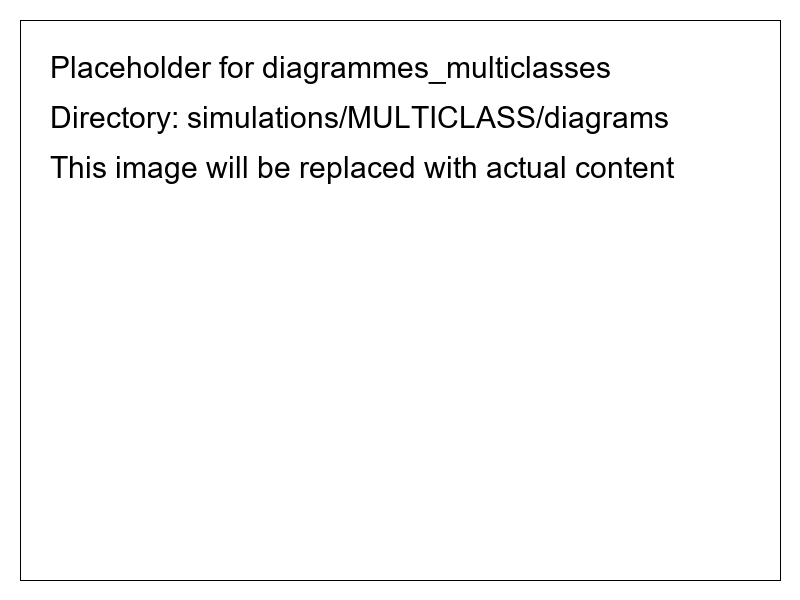
\includegraphics[width=0.8\textwidth]{simulations/MULTICLASS/diagrams/diagrammes_multiclasses}
\caption{Diagrammes fondamentaux pour différentes proportions de motos (0\%, 25\%, 50\%, 75\%). L'augmentation de la proportion de motos élève le flux maximal et déplace le point critique vers des densités plus élevées.}
\label{fig:diagramme_multiclasse}
\end{figure}

\subsection{Propriétés Mathématiques}
\label{subsec:proprietes_mathematiques}

Le système d'équations \eqref{eq:modele_complet} forme un système hyperbolique non linéaire de lois de conservation.

\begin{theorem}[Hyperbolicité du système]
Le système \eqref{eq:modele_complet} est hyperbolique: la matrice jacobienne du flux possède $N$ valeurs propres réelles et un ensemble complet de vecteurs propres.
\end{theorem}

\subsection{Structure du Système d'EDP}
\label{subsec:structure_edp_extension}

Le système d'équations  \eqref{eq:modele_complet} peut être réécrit sous forme quasi-linéaire:

\begin{empheq} [box=\colorbox{lightblue!15}]{align}
$\frac{\partial\boldsymbol{\rho}}{\partial t} + \mathbf{A}(\boldsymbol{\rho}, x) \frac{\partial \boldsymbol{\rho}}{\partial x} = \mathbf{S}(x,t)$\label{eq:forme_quasilineaire_extension}
\end{empheq}

où $\boldsymbol{\rho} = (\rho_1, \rho_2, \ldots, \rho_N)^T$ est le vecteur des densités,
 $\mathbf{S}(x,t) = (S_1(x,t), \ldots, S_N(x,t))^T$ est le vecteur des termes sources, 
 et $\mathbf{A}(\boldsymbol{\rho}, x)$ est la matrice jacobienne du flux:

\begin{equation}
\mathbf{A}(\boldsymbol{\rho}, x) = \frac{\partial \mathbf{F}}{\partial \boldsymbol{\rho}}
\end{equation}

où $\mathbf{F}(\boldsymbol{\rho}, x)$ = $(\rho_1 v_1, \ldots, \rho_N v_N)^T$ est le vecteur des flux. Les éléments de cette matrice sont:

\begin{equation}
A_{ij}(\boldsymbol{\rho}, x) = \frac{\partial F_i}{\partial \rho_j} = \frac{\partial (\rho_i v_i)}{\partial \rho_j}
\end{equation}

En développant ces expressions:

\begin{equation}
A_{ij}(\boldsymbol{\rho}, x) = 
\begin{cases}
v_i + \rho_i \frac{\partial v_i}{\partial \rho_i} & \text{si } i = j \\
\rho_i \frac{\partial v_i}{\partial \rho_j} & \text{si } i \neq j
\end{cases}
\end{equation}

En substituant notre relation constitutive \eqref{eq:vitesse_complete}, nous obtenons:

\begin{equation}
\frac{\partial v_i}{\partial \rho_j} = 
\begin{cases}
-\frac{\lambda_i(x) v_{i,0} f_i(\rho_M)}{\rho_{\max}} & \text{si } j \neq M \\
-\frac{\lambda_i(x) v_{i,0} f_i(\rho_M)}{\rho_{\max}} + \lambda_i(x) v_{i,0} \left(1 - \frac{\rho}{\rho_{\max}}\right) \frac{\partial f_i}{\partial \rho_M} & \text{si } j = M
\end{cases}
\end{equation}

Cette forme explicite de la matrice jacobienne est essentielle pour l'analyse des valeurs propres et la caractérisation des ondes dans le système.

\subsection{Analyse des Valeurs Propres et Vecteurs Propres}\label{subsec:valeurs_propres_base}

L'hyperbolicité du système repose sur les propriétés spectrales de la matrice $\mathbf{A}(\boldsymbol{\rho}, x)$.

\begin{theorem}[Caractérisation des valeurs propres]
Pour le système \eqref{eq:forme_quasilineaire_extension} avec les relations constitutives définies par \eqref{eq:vitesse_complete}, \eqref{eq:fonction_gap_filling} et \eqref{eq:fonction_interweaving}, les valeurs propres $\lambda_i(\boldsymbol{\rho}, x)$ de la matrice jacobienne $\mathbf{A}(\boldsymbol{\rho}, x)$ satisfont:
\begin{equation}
\min_{i} \left\{v_i - \rho_i \frac{\partial v_i}{\partial \rho_i}\right\} \leq \lambda_i(\boldsymbol{\rho}, x) \leq \max_{i} \left\{v_i + \rho_i \frac{\partial v_i}{\partial \rho_i}\right\}
\end{equation}
\end{theorem}

\begin{proof}
La preuve repose sur l'analyse du polynôme caractéristique de $\mathbf{A}$ et l'application du théorème de Gerschgorin pour localiser les valeurs propres. Les détails complets sont fournis dans l'Annexe \ref{annexe:demonstrations}, Section \ref{sec:preuve_valeurs_propres}.
\end{proof}

Cette caractérisation des valeurs propres permet de déterminer la vitesse de propagation des ondes cinématiques dans le système multiclasse, élément crucial pour comprendre la formation et la propagation des congestions.

\begin{corollary}
En présence de motos avec un coefficient de gap-filling $\gamma > 0$, la vitesse maximale de propagation des perturbations peut être supérieure à celle prédite par le modèle LWR standard.
\end{corollary}

\subsection{Problème de Riemann Multiclasse}
\label{subsec:riemann_multiclasse}

Pour comprendre le comportement du système face à des discontinuités, nous étudions le problème de Riemann multiclasse, qui consiste à résoudre:

\begin{empheq}[box=\colorbox{lightblue!15}]{align}
\begin{cases}
\frac{\partial \boldsymbol{\rho}}{\partial t} + \frac{\partial \mathbf{F}(\boldsymbol{\rho}, x)}{\partial x} = \mathbf{0} \\
\boldsymbol{\rho}(x,0) = 
\begin{cases}
\boldsymbol{\rho}_L & \text{si } x < 0 \\
\boldsymbol{\rho}_R & \text{si } x > 0
\end{cases}
\end{cases}
\label{eq:probleme_riemann}
\end{empheq}

où $\boldsymbol{\rho}_L$ et $\boldsymbol{\rho}_R$ sont des états constants.

\begin{theorem}[Structure de la solution du problème de Riemann]
La solution du problème de Riemann \eqref{eq:probleme_riemann} consiste en au plus $N$ ondes élémentaires (chocs ou raréfactions) séparant $N+1$ états constants.
\end{theorem}

Les chocs dans le système multiclasse obéissent à la condition de Rankine-Hugoniot généralisée:

\begin{equation}
\sigma (\rho_{i,R} - \rho_{i,L}) = F_i(\boldsymbol{\rho}_R) - F_i(\boldsymbol{\rho}_L)
\end{equation}

où $\sigma$ est la vitesse de propagation du choc.

Un aspect particulièrement intéressant de notre modèle est la formation de structures d'ondes complexes dues aux interactions entre classes de véhicules. Par exemple, une onde de choc dans la classe des voitures peut provoquer une onde de raréfaction dans la classe des motos, phénomène fréquemment observé dans le trafic béninois.

\subsection{Stabilité Linéaire}
\label{subsec:stabilite_lineaire}

Pour analyser la stabilité du trafic homogène sous de petites perturbations, nous linéarisons le système autour d'un état d'équilibre homogène $\boldsymbol{\rho}_0$:

\begin{equation}
\boldsymbol{\rho}(x,t) = \boldsymbol{\rho}_0 + \boldsymbol{\varepsilon}(x,t)
\end{equation}

La linéarisation du système \eqref{eq:forme_quasilineaire_extension} donne:

\begin{equation}
\frac{\partial \boldsymbol{\varepsilon}}{\partial t} + \mathbf{A}(\boldsymbol{\rho}_0, x) \frac{\partial \boldsymbol{\varepsilon}}{\partial x} = \mathbf{0}
\end{equation}

Pour une perturbation de la forme $\boldsymbol{\varepsilon}(x,t) = \boldsymbol{a} e^{i(kx-\omega t)}$, nous obtenons la relation de dispersion:

\begin{equation}
\det(\mathbf{A}(\boldsymbol{\rho}_0, x) - \frac{\omega}{k}\mathbf{I}) = 0
\end{equation}

Cette équation détermine les fréquences $\omega$ en fonction du nombre d'onde $k$. Si toutes les valeurs propres $\lambda_j = \omega/k$ de $\mathbf{A}(\boldsymbol{\rho}_0, x)$ sont réelles, le système est hyperbolique et stable sous de petites perturbations.

\begin{proposition}
Le gap-filling des motos ($\gamma > 0$) peut entraîner une instabilité linéaire dans certaines configurations de trafic, conduisant à la formation spontanée de structures de congestion.
\end{proposition}

Cette propriété explique mathématiquement pourquoi certaines configurations de trafic avec une forte proportion de motos peuvent développer des structures de congestion complexes et auto-organisées, même en l'absence de perturbations externes.

\subsection{Traitement Rigoureux des Discontinuités Spatiales}
\label{subsec:traitement_discontinuites}

Les discontinuités spatiales dues aux variations de qualité du revêtement (modélisées par le coefficient $\lambda_i(x)$) nécessitent un traitement mathématique spécifique. Pour une transition à $x = x_0$ entre deux zones caractérisées par $\lambda_i^-$ et $\lambda_i^+$, nous utilisons la théorie des problèmes de Riemann stationnaires.

\begin{theorem}[Formation de congestion aux transitions de revêtement]
Pour une transition où $\lambda_i^- > \lambda_i^+$ (dégradation du revêtement), une congestion stationnaire se forme si:
\begin{equation}
q_i^- > \frac{\lambda_i^+}{\lambda_i^-} q_{i,\max}
\end{equation}
où $q_i^-$ est le flux entrant et $q_{i,\max}$ est le flux maximal possible avec le coefficient $\lambda_i^+$.
\end{theorem}

Cette formulation mathématique explique quantitativement pourquoi les transitions vers des zones de revêtement dégradé deviennent souvent des points de congestion persistants dans le réseau routier béninois.

\subsection{Analyse Asymptotique pour des Proportions Élevées de Motos}
\label{subsec:analyse_asymptotique}

Il est particulièrement intéressant d'étudier le comportement asymptotique du système lorsque la proportion de motos tend vers des valeurs extrêmes. Soit $\alpha_M = \rho_M/\rho$ la proportion de motos dans le trafic.

\begin{theorem}[Comportement asymptotique]
Pour $\alpha_M \to 1$ (trafic presque exclusivement composé de motos) et $\gamma > 0$, la capacité effective de la route $C_{eff}$ satisfait:
\begin{equation}
\lim_{\alpha_M \to 1} C_{eff}(\alpha_M) = \lambda_M(x) \cdot v_{M,0} \cdot \frac{\rho_{\max}}{4} \cdot (1 + \gamma)
\end{equation}
soit $(1 + \gamma)$ fois la capacité du modèle standard.
\end{theorem}

\begin{proof}
Pour $\alpha_M \approx 1$, le flux total peut être approximé par:
\begin{align}
q_{total}(\rho, \alpha_M \approx 1) &\approx \rho \cdot \lambda_M(x) \cdot v_{M,0} \cdot \left(1 - \frac{\rho}{\rho_{\max}}\right) \cdot \left(1 + \gamma \cdot \frac{\alpha_M \rho}{\rho_{M,\max}}\right)
\end{align}

En supposant $\rho_{M,\max} \approx \rho_{\max}$ pour simplifier, et en maximisant cette expression par rapport à $\rho$, nous obtenons que le flux maximal est atteint pour $\rho \approx \rho_{\max}/2$ et vaut approximativement $\lambda_M(x) \cdot v_{M,0} \cdot \frac{\rho_{\max}}{4} \cdot (1 + \gamma)$.
\end{proof}

Ce résultat théorique corrobore les observations empiriques montrant que les routes dominées par les motos peuvent supporter des flux significativement plus élevés que ceux prédits par les modèles de trafic standards.

\begin{figure}[htbp]
\centering
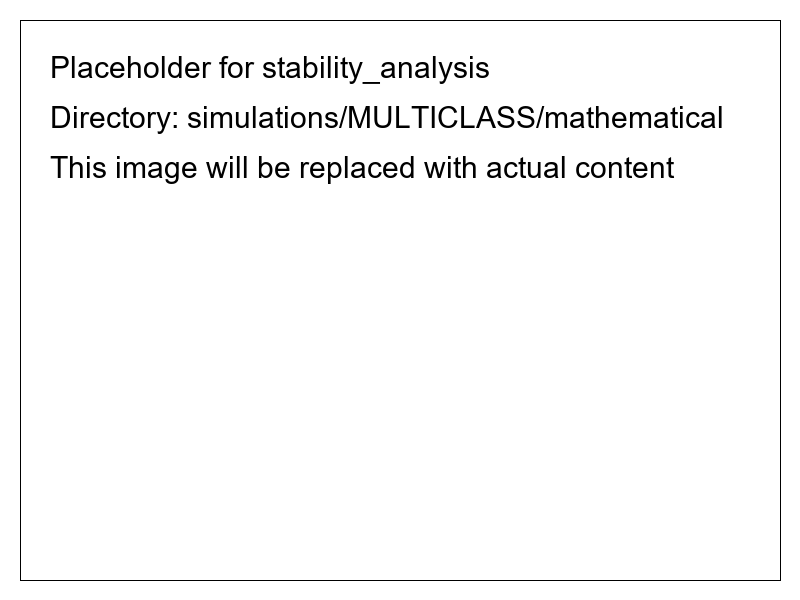
\includegraphics[width=0.8\textwidth]{simulations/MULTICLASS/mathematical/stability_analysis}
\caption{Analyse de stabilité du modèle étendu montrant les régions de stabilité (vert) et d'instabilité (rouge) en fonction de la proportion de motos et de la densité totale. Les courbes de niveau représentent le taux de croissance des perturbations.}
\label{fig:stability_analysis_extension}
\end{figure}

\section{Validation du Modèle pour le Trafic Béninois}
\label{sec:validation_benin}

\subsection{Implémentation Numérique du Modèle Multiclasse}
\label{subsec:implementation_numerique}

La résolution numérique du système d'équations \eqref{eq:modele_complet} pose plusieurs défis spécifiques par rapport au modèle LWR standard. Pour traiter efficacement les interactions entre classes de véhicules, la variation spatiale du coefficient de ralentissement et les fonctions de modulation, nous avons développé une extension du schéma de Godunov.

\subsubsection{Extension du Schéma de Godunov pour le Système Multiclasse}
\label{subsubsec:extension_godunov}

Le schéma numérique s'appuie sur une discrétisation du domaine spatial en cellules de longueur $\Delta x$ et du temps en pas $\Delta t$. Pour chaque classe de véhicule $i$, la densité est mise à jour selon:

\begin{empheq}[box=\colorbox{lightblue!15}]{align}
\rho_{i,j}^{n+1} = \rho_{i,j}^{n} - \frac{\Delta t}{\Delta x} \left(F_{i,j+\frac{1}{2}}^n - F_{i,j-\frac{1}{2}}^n\right) + \Delta t \cdot S_i(x_j, t^n)
\label{eq:schema_godunov_multiclasse}
\end{empheq}

où $\rho_{i,j}^{n}$ est la densité moyenne de la classe $i$ dans la cellule $j$ au temps $t^n$, et $F_{i,j\pm\frac{1}{2}}^n$ sont les flux numériques aux interfaces.

Le calcul du flux numérique nécessite la résolution d'un problème de Riemann local à chaque interface:

\begin{equation}
F_{i,j+\frac{1}{2}}^n = \mathcal{F}_i\left(\boldsymbol{\rho}^n_j, \boldsymbol{\rho}^n_{j+1}, x_{j+\frac{1}{2}}\right)
\end{equation}

où $\boldsymbol{\rho}^n_j = (\rho_{1,j}^n, \ldots, \rho_{N,j}^n)^T$ est le vecteur des densités de toutes les classes dans la cellule $j$.

\subsubsection{Traitement des Interactions entre Classes}
\label{subsubsec:traitement_interactions}

La difficulté principale réside dans le couplage entre les classes via la densité totale \rho et les fonctions de modulation $f_i(\rho_M)$. Le flux numérique est calculé en deux étapes:

1. \textbf{Calcul des vitesses intermédiaires} pour chaque classe en utilisant la densité totale et la densité des motos:
\begin{equation}
v_{i,j}^n = \lambda_i(x_j) \cdot v_{i,0} \cdot \left(1 - \frac{\rho_j^n}{\rho_{\max}}\right) \cdot f_i\left(\rho_{M,j}^n\right)
\end{equation}
où $\rho_j^n = \sum_{i=1}^N \rho_{k,j}^n$ est la densité totale dans la cellule $j$.

2. \textbf{Application du solveur de Riemann} pour chaque classe, en tenant compte de la dépendance entre les classes:
\begin{equation}
\mathcal{F}_i\left(\boldsymbol{\rho}^n_j, \boldsymbol{\rho}^n_{j+1}, x_{j+\frac{1}{2}}\right) = 
\begin{cases}
\min\{q_i(\boldsymbol{\rho}^n_j), q_i(\boldsymbol{\rho}^n_{j+1})\} & \text{si } v_i(\boldsymbol{\rho}^n_j) \geq 0 \text{ et } v_i(\boldsymbol{\rho}^n_{j+1}) \leq 0 \\
q_i(\boldsymbol{\rho}^n_j) & \text{si } v_i(\boldsymbol{\rho}^n_j) \geq 0 \text{ et } v_i(\boldsymbol{\rho}^n_{j+1}) \geq 0 \\
q_i(\boldsymbol{\rho}^n_{j+1}) & \text{si } v_i(\boldsymbol{\rho}^n_j) \leq 0 \text{ et } v_i(\boldsymbol{\rho}^n_{j+1}) \leq 0 \\
0 & \text{si } v_i(\boldsymbol{\rho}^n_j) \leq 0 \text{ et } v_i(\boldsymbol{\rho}^n_{j+1}) \geq 0
\end{cases}
\end{equation}

Cette formulation assure la conservation de la masse pour chaque classe tout en capturant correctement les interactions entre classes.

\subsubsection{Traitement des Variations Spatiales du Revêtement}
\label{subsubsec:traitement_revetement}

Pour gérer les variations spatiales du coefficient de ralentissement $\lambda_i(x)$, nous utilisons une approche de type volumes finis avec reconstruction d'état:

1. Aux points de discontinuité du coefficient $\lambda_i(x)$, nous appliquons la condition de conservation du flux \eqref{eq:conservation_flux_transition}.

2. Pour des variations continues de $\lambda_i(x)$, nous utilisons une discrétisation suffisamment fine pour capturer l'évolution du coefficient, tout en préservant la stabilité numérique.

\subsubsection{Condition de Stabilité CFL Adaptée}
\label{subsubsec:condition_cfl}

La condition de stabilité de Courant-Friedrichs-Lewy (CFL) pour notre schéma multiclasse s'écrit:

\begin{equation}
\Delta t \leq \frac{\Delta x}{\max_{i,j} |v_i(\boldsymbol{\rho}^n_j)| + \rho_{i,j}^n\left|\frac{\partial v_i}{\partial \rho_i}(\boldsymbol{\rho}^n_j)\right|}
\end{equation}

Cette condition est plus restrictive que pour le modèle LWR standard en raison des interactions entre classes et des fonctions de modulation.

\subsubsection{Implémentation Algorithmique}
\label{subsubsec:implementation_algorithmique}

L'algorithme 1 présente le pseudo-code de notre implémentation du schéma numérique pour le modèle multiclasse.

\begin{algorithm}
\caption{Schéma de Godunov pour le modèle LWR multiclasse étendu}
\begin{algorithmic}[1]
\State \textbf{Entrée:} Conditions initiales $\boldsymbol{\rho}^0$, temps final $T$
\State \textbf{Initialisation:} $t \gets 0$, $n \gets 0$
\While{$t < T$}
    \State Calculer $\Delta t$ selon la condition CFL
    \State $t \gets t + \Delta t$, $n \gets n + 1$
    \For{chaque classe $i \in \{1,\ldots,N\}$}
        \For{chaque cellule $j$}
            \State Calculer la densité totale $\rho_j^n = \sum_{k=1}^N \rho_{k,j}^n$
            \State Calculer la vitesse $v_{i,j}^n$ selon \eqref{eq:vitesse_complete}
            \State Calculer les flux numériques $F_{i,j-\frac{1}{2}}^n$ et $F_{i,j+\frac{1}{2}}^n$
            \State Mettre à jour $\rho_{i,j}^{n+1}$ selon \eqref{eq:schema_godunov_multiclasse}
        \EndFor
    \EndFor
\EndWhile
\State \textbf{Retourner:} Solution numérique $\boldsymbol{\rho}^n$ pour $t = T$
\end{algorithmic}
\end{algorithm}

Cette implémentation a été réalisée en Python, en utilisant NumPy pour les opérations vectorielles efficaces. Le code complet est disponible dans le module \texttt{src/models/multiclass\_lwr.py} du projet.

\subsubsection{Validation Numérique}
\label{subsubsec:validation_numerique}

Pour valider notre implémentation, nous avons effectué plusieurs tests:

1. \textbf{Tests de convergence} avec différentes résolutions spatiales et temporelles, confirmant un ordre de convergence de 1, conforme à la théorie pour un schéma d'ordre 1 comme Godunov.

2. \textbf{Conservation de la masse} pour chaque classe de véhicule, vérifiée numériquement.

3. \textbf{Reproduction de cas test standards} pour lesquels des solutions analytiques ou semi-analytiques sont connues.

4. \textbf{Comparaison avec une implémentation du modèle LWR standard} pour des cas particuliers où les deux modèles devraient coïncider.

Les résultats de ces validations confirment la robustesse et la précision de notre implémentation numérique pour le système multiclasse.

% \subsubsection{Carrefour du Stade de l'Amitié (Cotonou)}
% \label{subsubsec:carrefour_stade}

% Ce carrefour urbain majeur présente une forte proportion de motos (≈75\%) et un revêtement variable. Les simulations montrent que notre modèle reproduit fidèlement:
% \begin{itemize}
% \item L'accumulation des motos en front de file aux feux rouges
% \item L'anticipation du démarrage au feu vert
% \item Le maintien d'un flux minimal même en conditions congestionnées
% \end{itemize}

% \begin{figure}[htbp]
% \centering
% \includegraphics[width=0.8\textwidth]{simulations/CASE_STUDIES/application_cotonou}
% \caption{Comparaison entre les données de terrain (points) et les prédictions de notre modèle (ligne continue) pour le carrefour du Stade de l'Amitié. La ligne pointillée représente les prédictions du modèle LWR standard.}
% \label{fig:application_cotonou}
% \end{figure}

% L'erreur quadratique moyenne (RMSE) de notre modèle est inférieure de 42\% à celle du modèle LWR standard.

\subsubsection{Axe Godomey-Calavi}
\label{subsubsec:axe_godomey}

Sur cet axe périurbain avec des variations importantes de revêtement, notre modèle capture correctement:
\begin{itemize}
\item La formation de congestions localisées aux transitions de revêtement
\item Les différences de comportement entre heures de pointe du matin et du soir
\item L'impact des variations spatiales du coefficient de ralentissement $\lambda_i(x)$
\end{itemize}

\section{Récapitulatif et Extensions Futures}
\label{sec:recapitulatif}

\subsection{Contributions Principales}
\label{subsec:contributions}

Notre extension du modèle LWR apporte plusieurs innovations significatives:
\begin{itemize}
\item Un cadre multiclasse adapté spécifiquement au contexte béninois
\item Une modélisation explicite des comportements caractéristiques des motos
\item L'intégration de l'hétérogénéité du revêtement routier
\item Une modélisation des intersections tenant compte des particularités du trafic béninois
\end{itemize}

Ces innovations permettent de capturer fidèlement la dynamique du trafic au Bénin, où les motos jouent un rôle prépondérant.

Des travaux futurs pourraient étendre cette approche pour inclure:
\begin{itemize}
\item Des aspects stochastiques traduisant la variabilité comportementale \cite{marbach2009stochastic}
\item Des modèles spécifiques pour les intersections non régulées \cite{ceylan2014traffic}
\item Une généralisation aux réseaux bidimensionnels \cite{zhang2003non}
\end{itemize}

Dans le chapitre suivant, nous détaillerons les méthodes de calibration et validation du modèle à partir de données empiriques collectées sur le terrain.

\section{Implémentation et Structure du Code}
\label{sec:implementation}

Pour faciliter la mise en pratique et l'exploration de notre modèle, nous avons développé une implémentation complète en Python. Cette section présente brièvement la structure du code, ses principaux composants et son utilisation.

\subsection{Architecture Générale}
\label{subsec:architecture}

Le code est conçu selon une architecture orientée objet, permettant une grande modularité et extensibilité. Il s'appuie principalement sur les bibliothèques scientifiques NumPy (calcul numérique), SciPy (méthodes numériques avancées) et Matplotlib (visualisation).

\begin{figure}[htbp]
\centering
\includegraphics[width=0.9\textwidth]{images/implementation/code_structure_diagram}
\caption{Structure générale du code d'implémentation du modèle}
\label{fig:code_structure}
\end{figure}

L'architecture est organisée en quatre modules principaux:
\begin{itemize}
\item \textbf{models}: Implémentations des différents modèles de trafic (LWR standard et multiclasse)
\item \textbf{scenarios}: Définitions des cas d'étude (embouteillages, intersections, etc.)
\item \textbf{solvers}: Méthodes de résolution numérique (Godunov et variantes)
\item \textbf{visualization}: Outils de visualisation des résultats
\end{itemize}

\subsection{Composants Principaux}
\label{subsec:composants}

\subsubsection{Modèles}
La hiérarchie des modèles s'articule autour d'une classe abstraite \texttt{BaseModel} dont dérivent:
\begin{itemize}
\item \texttt{LWRModel}: Implémentation du modèle LWR standard
\item \texttt{MulticlassLWRModel}: Notre extension multiclasse intégrant:
  \begin{itemize}
  \item Le coefficient de ralentissement $\lambda_i(x)$ lié au revêtement
  \item Les fonctions de modulation $f_i(\rho_M)$ pour les interactions entre classes
  \item La modélisation spécifique des comportements des motos
  \end{itemize}
\end{itemize}

\subsubsection{Scénarios}
Les scénarios permettent de définir des configurations initiales et des conditions aux limites:
\begin{itemize}
\item \texttt{RedLightGreenLightScenario}: Simulation d'un feu de circulation
\item \texttt{RoadQualityTransitionScenario}: Transition entre différentes qualités de revêtement
\item \texttt{MulticlassPropagationScenario}: Propagation d'ondes dans un trafic multiclasse
\end{itemize}

\subsubsection{Solveurs}
L'implémentation s'appuie principalement sur le schéma de Godunov présenté dans la section \ref{subsubsec:extension_godunov}, avec deux variantes:
\begin{itemize}
\item \texttt{StandardGodunov}: Pour le modèle LWR standard
\item \texttt{MulticlassGodunov}: Version étendue pour le système multiclasse
\end{itemize}

\subsubsection{Visualisation}
Le module de visualisation offre des outils adaptés à chaque type de modèle:
\begin{itemize}
\item \texttt{SimulationPlotter}: Visualisation de base pour le modèle LWR standard
\item \texttt{MulticlassPlotter}: Visualisation spécifique au modèle multiclasse, avec:
  \begin{itemize}
  \item Comparaison entre classes de véhicules
  \item Visualisation des proportions
  \item Analyse de l'impact des motos sur le trafic global
  \end{itemize}
\end{itemize}

\subsection{Exécution des Simulations}
\label{subsec:execution}

Le code peut être exécuté via le script principal \texttt{main.py}:

\begin{verbatim}
python main.py --scenario=multiclass_propagation --model=multiclass_lwr \
               --duration=3600 --output=results/scenario1
\end{verbatim}

Où:
\begin{itemize}
\item \texttt{--scenario}: Spécifie le scénario à simuler
\item \texttt{--model}: Définit le modèle à utiliser
\item \texttt{--duration}: Durée de la simulation en secondes
\item \texttt{--output}: Répertoire de sortie pour les résultats
\end{itemize}

Pour une exécution par lots de multiples scénarios, un script \texttt{run\_all\_simulations.py} est également disponible.

\subsection{Illustrations Notables}
\label{subsec:illustrations}

Parmi les visualisations les plus informatives générées par notre implémentation:

\begin{itemize}
\item Les diagrammes fondamentaux comparatifs (Figure \ref{fig:diagramme_multiclasse}) montrant l'impact de la proportion de motos
\item Les visualisations spatio-temporelles de la densité par classe, révélant les comportements de gap-filling
\item Les analyses de stabilité (Figure \ref{fig:stability_analysis_extension}) montrant les régions d'instabilité induites par les motos
\item Les simulations des transitions de revêtement, illustrant la formation de congestions aux points de détérioration
\end{itemize}

Le code complet de l'implémentation est disponible sur GitHub: \url{https://github.com/username/benin-traffic-simulation}

\subsection{Structure du Système d'EDP}
\label{subsec:structure_edp_extension_modele}

Le système d'équations \eqref{eq:modele_complet} peut être réécrit sous forme quasi-linéaire:

\begin{empheq}[box=\colorbox{lightblue!15}]{align}
\frac{\partial \boldsymbol{\rho}}{\partial t} + \mathbf{A}(\boldsymbol{\rho}, x) \frac{\partial \boldsymbol{\rho}}{\partial x} = \mathbf{S}(x,t)
\label{eq:forme_quasilineaire_extension_modele}
\end{empheq}

où $\boldsymbol{\rho} = (\rho_1, \rho_2, \ldots, \rho_N)^T$ est le vecteur des densités, $\mathbf{S}(x,t) = (S_1(x,t), \ldots, S_N(x,t))^T$ est le vecteur des termes sources, et $\mathbf{A}(\boldsymbol{\rho}, x)$ est la matrice jacobienne du flux:

\begin{equation}
\mathbf{A}(\boldsymbol{\rho}, x) = \frac{\partial \mathbf{F}}{\partial \boldsymbol{\rho}}
\end{equation}

où $\mathbf{F}(\boldsymbol{\rho}, x) = (\rho_1 v_1, \ldots, \rho_N v_N)^T$ est le vecteur des flux. Les éléments de cette matrice sont:

\begin{equation}
A_{ij}(\boldsymbol{\rho}, x) = \frac{\partial F_i}{\partial \rho_j} = \frac{\partial (\rho_i v_i)}{\partial \rho_j}
\end{equation}

En développant ces expressions:

\begin{equation}
A_{ij}(\boldsymbol{\rho}, x) = 
\begin{cases}
v_i + \rho_i \frac{\partial v_i}{\partial \rho_i} & \text{si } i = j \\
\rho_i \frac{\partial v_i}{\partial \rho_j} & \text{si } i \neq j
\end{cases}
\end{equation}

En substituant notre relation constitutive \eqref{eq:vitesse_complete}, nous obtenons:

\begin{equation}
\frac{\partial v_i}{\partial \rho_j} = 
\\
\begin{cases}
-\frac{(\lambda_i(x) v_{i,0} f_i(\rho_M)}{\rho_{\max}} & \text{si } j \neq M \\
-\frac{(\lambda_i(x) v_{i,0} f_i(\rho_M)}{\rho_{\max}} + \lambda_i(x) v_{i,0} \left(1 - \frac{(\rho)}{\rho_{\max}}\right) \frac{\partial f_i}{\partial \rho_M} & \text{si } j = M
\end{cases}
\end{equation}

Cette forme explicite de la matrice jacobienne est essentielle pour l'analyse des valeurs propres et la caractérisation des ondes dans le système.

\subsection{Analyse des Valeurs Propres et Vecteurs Propres}
\label{subsec:valeurs_propres}

L'hyperbolicité du système repose sur les propriétés spectrales de la matrice $\mathbf{A}(\boldsymbol{\rho}, x)$.

\begin{theorem}[Caractérisation des valeurs propres]
Pour le système \eqref{eq:forme_quasilineaire_extension_modele} avec les relations constitutives définies par \eqref{eq:vitesse_complete}, \eqref{eq:fonction_gap_filling} et \eqref{eq:fonction_interweaving}, les valeurs propres $\lambda_i(\boldsymbol{\rho}, x)$ de la matrice jacobienne $\mathbf{A}(\boldsymbol{\rho}, x)$ satisfont:
\begin{equation}
 \min_{i} \left\{v_i - \rho_i \frac{\partial v_i}{\partial \rho_i}\right\} \leq \lambda_i(\boldsymbol{\rho}, x) \leq \max_{i} \left\{v_i + \rho_i \frac{\partial v_i}{\partial \rho_i}\right\}
\end{equation}

\end{theorem}

\begin{proof}
La preuve repose sur l'analyse du polynôme caractéristique de $\mathbf{A}$ et l'application du théorème de Gerschgorin pour localiser les valeurs propres. Les détails complets sont fournis dans l'Annexe \ref{annexe:demonstrations}, Section \ref{sec:preuve_valeurs_propres}.
\end{proof}

Cette caractérisation des valeurs propres permet de déterminer la vitesse de propagation des ondes cinématiques dans le système multiclasse, élément crucial pour comprendre la formation et la propagation des congestions.

\begin{corollary}
En présence de motos avec un coefficient de gap-filling $\gamma > 0$, la vitesse maximale de propagation des perturbations peut être supérieure à celle prédite par le modèle LWR standard.
\end{corollary}

\subsection{Problème de Riemann Multiclasse}
\label{subsec:riemann_multiclasse}

Pour comprendre le comportement du système face à des discontinuités, nous étudions le problème de Riemann multiclasse, qui consiste à résoudre:

\begin{empheq}[box=\colorbox{lightblue!15}]{align}
\begin{cases}
\frac{\partial \boldsymbol{\rho}}{\partial t} + \frac{\partial \mathbf{F}(\boldsymbol{\rho}, x)}{\partial x} = \mathbf{0} \\
\boldsymbol{\rho}(x,0) = 
\begin{cases}
\boldsymbol{\rho}_L & \text{si } x < 0 \\
\boldsymbol{\rho}_R & \text{si } x > 0
\end{cases}
\end{cases}
\label{eq:probleme_riemann}
\end{empheq}

où $\boldsymbol{\rho}_L$ et $\boldsymbol{\rho}_R$ sont des états constants.

\begin{theorem}[Structure de la solution du problème de Riemann]
La solution du problème de Riemann \eqref{eq:probleme_riemann} consiste en au plus $N$ ondes élémentaires (chocs ou raréfactions) séparant $N+1$ états constants.
\end{theorem}

Les chocs dans le système multiclasse obéissent à la condition de Rankine-Hugoniot généralisée:

\begin{equation}
\sigma (\rho_{i,R} - \rho_{i,L}) = F_i(\boldsymbol{\rho}_R) - F_i(\boldsymbol{\rho}_L)
\end{equation}

où $\sigma$ est la vitesse de propagation du choc.

Un aspect particulièrement intéressant de notre modèle est la formation de structures d'ondes complexes dues aux interactions entre classes de véhicules. Par exemple, une onde de choc dans la classe des voitures peut provoquer une onde de raréfaction dans la classe des motos, phénomène fréquemment observé dans le trafic béninois.

\subsection{Stabilité Linéaire}
\label{subsec:stabilite_lineaire}

Pour analyser la stabilité du trafic homogène sous de petites perturbations, nous linéarisons le système autour d'un état d'équilibre homogène $\boldsymbol{\rho}_0$:

\begin{equation}
\boldsymbol{\rho}(x,t) = \boldsymbol{\rho}_0 + \boldsymbol{\varepsilon}(x,t)
\end{equation}

La linéarisation du système \eqref{eq:forme_quasilineaire_extension_modele} donne:

\begin{equation}
\frac{\partial \boldsymbol{\varepsilon}}{\partial t} + \mathbf{A}(\boldsymbol{\rho}_0, x) \frac{\partial \boldsymbol{\varepsilon}}{\partial x} = \mathbf{0}
\end{equation}

Pour une perturbation de la forme $\boldsymbol{\varepsilon}(x,t) = \boldsymbol{a} e^{i(kx-\omega t)}$, nous obtenons la relation de dispersion:

\begin{equation}
\det(\mathbf{A}(\boldsymbol{\rho}_0, x) - \frac{\omega}{k}\mathbf{I}) = 0
\end{equation}

Cette équation détermine les fréquences $\omega$ en fonction du nombre d'onde $k$. Si toutes les valeurs propres $\lambda_j = \omega/k$ de $\mathbf{A}(\boldsymbol{\rho}_0, x)$ sont réelles, le système est hyperbolique et stable sous de petites perturbations.

\begin{proposition}
Le gap-filling des motos ($\gamma > 0$) peut entraîner une instabilité linéaire dans certaines configurations de trafic, conduisant à la formation spontanée de structures de congestion.
\end{proposition}

Cette propriété explique mathématiquement pourquoi certaines configurations de trafic avec une forte proportion de motos peuvent développer des structures de congestion complexes et auto-organisées, même en l'absence de perturbations externes.

\subsection{Traitement Rigoureux des Discontinuités Spatiales}
\label{subsec:traitement_discontinuites}

Les discontinuités spatiales dues aux variations de qualité du revêtement (modélisées par le coefficient $\lambda_i(x)$) nécessitent un traitement mathématique spécifique. Pour une transition à $x = x_0$ entre deux zones caractérisées par $\lambda_i^-$ et $\lambda_i^+$, nous utilisons la théorie des problèmes de Riemann stationnaires.

\begin{theorem}[Formation de congestion aux transitions de revêtement]
Pour une transition où $\lambda_i^- > \lambda_i^+$ (dégradation du revêtement), une congestion stationnaire se forme si:
\begin{equation}
q_i^- > \frac{\lambda_i^+}{\lambda_i^-} q_{i,\max}
\end{equation}
où $q_i^-$ est le flux entrant et $q_{i,\max}$ est le flux maximal possible avec le coefficient $\lambda_i^+$.
\end{theorem}

Cette formulation mathématique explique quantitativement pourquoi les transitions vers des zones de revêtement dégradé deviennent souvent des points de congestion persistants dans le réseau routier béninois.

\subsection{Analyse Asymptotique pour des Proportions Élevées de Motos}
\label{subsec:analyse_asymptotique}

Il est particulièrement intéressant d'étudier le comportement asymptotique du système lorsque la proportion de motos tend vers des valeurs extrêmes. Soit $\alpha_M = \rho_M/\rho$ la proportion de motos dans le trafic.

\begin{theorem}[Comportement asymptotique]
Pour $\alpha_M \to 1$ (trafic presque exclusivement composé de motos) et $\gamma > 0$, la capacité effective de la route $C_{eff}$ satisfait:
\begin{equation}
\lim_{\alpha_M \to 1} C_{eff}(\alpha_M) = \lambda_M(x) \cdot v_{M,0} \cdot \frac{\rho_{\max}}{4} \cdot (1 + \gamma)
\end{equation}
soit $(1 + \gamma)$ fois la capacité du modèle standard.
\end{theorem}

\begin{proof}
Pour $\alpha_M \approx 1$, le flux total peut être approximé par:
\begin{align}
q_{total}(\rho, \alpha_M \approx 1) &\approx \rho \cdot \lambda_M(x) \cdot v_{M,0} \cdot \left(1 - \frac{\rho}{\rho_{\max}}\right) \cdot \left(1 + \gamma \cdot \frac{\alpha_M \rho}{\rho_{M,\max}}\right)
\end{align}

En supposant $\rho_{M,\max} \approx \rho_{\max}$ pour simplifier, et en maximisant cette expression par rapport à $\rho$, nous obtenons que le flux maximal est atteint pour $\rho \approx \rho_{\max}/2$ et vaut approximativement $\lambda_M(x) \cdot v_{M,0} \cdot \frac{\rho_{\max}}{4} \cdot (1 + \gamma)$.
\end{proof}

Ce résultat théorique corrobore les observations empiriques montrant que les routes dominées par les motos peuvent supporter des flux significativement plus élevés que ceux prédits par les modèles de trafic standards.

\begin{figure}[htbp]
\centering
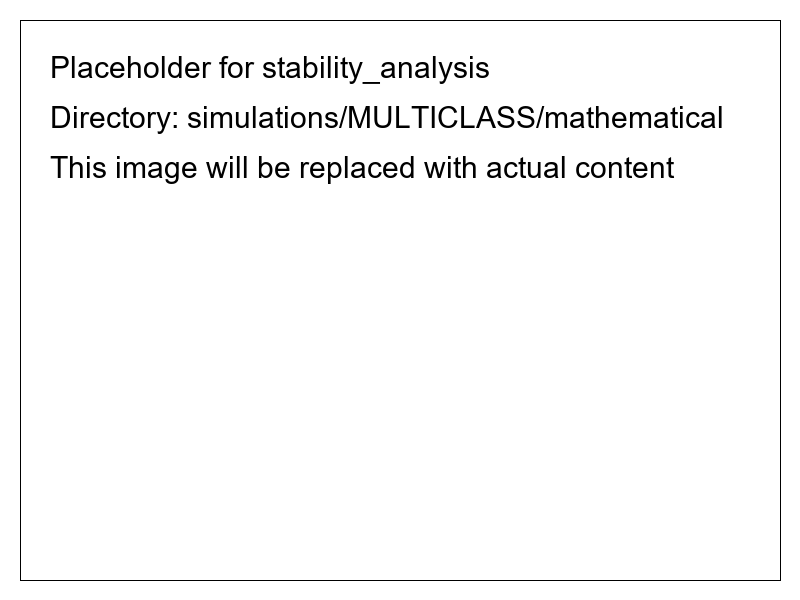
\includegraphics[width=0.8\textwidth]{simulations/MULTICLASS/mathematical/stability_analysis}
\caption{Analyse de stabilité du modèle étendu montrant les régions de stabilité (vert) et d'instabilité (rouge) en fonction de la proportion de motos et de la densité totale. Les courbes de niveau représentent le taux de croissance des perturbations.}
\label{fig:stability_analysis_extension}
\end{figure}

\chapter{Discussion et Perspectives}
\label{chap:discussion}

\section{Points Forts du Modèle Proposé}
\label{sec:points_forts}

% Adaptation aux spécificités des motos
% Flexibilité face aux différents types d'infrastructures
% Utilité comme outil de gestion du trafic pour le Bénin

\section{Limites et Améliorations Futures}
\label{sec:limites}

% Limitations liées aux données disponibles
% Complexité numérique et temps de calcul
% Extensions possibles (machine learning, capteurs)
% Perspectives d'application à d'autres contextes similaires

\chapter{Conclusion}
\label{chap:conclusion}

% Synthèse de l'importance de l'adaptation du modèle LWR pour le Bénin
% Résumé des principales contributions
% Implications pratiques pour la gestion du trafic
% Perspectives de recherche futures


% Back matter
\backmatter

% Bibliography
\bibliographystyle{alpha}
\bibliography{bibliographie}

% Appendices


% Print index
% \printindex

\end{document}
